% \documentclass[A4, 12pt]{article}
\documentclass[11pt]{article}

% Page setup
\usepackage[a4paper, left=1.5in, right=1in, top=1in, bottom=1in]{geometry}

% Spacing and indentation
\usepackage{setspace}
\setlength{\parindent}{0.25in} 
\setlength{\parskip}{0pt} 
\doublespacing


% Math and graphics
\usepackage{graphicx}
\usepackage{amsmath}
\usepackage{array}

% Tables
\usepackage{multirow}
\usepackage{booktabs}
\usepackage{float}


% Bibliography
\usepackage[backend=biber,style=apa]{biblatex}
\addbibresource{references.bib}

\usepackage{titlesec}
\usepackage{titletoc}
\usepackage{url}

% test

% Add this to your preamble:
\usepackage{tikz}
\usetikzlibrary{shapes.geometric, arrows, positioning}

% Define styles
\tikzstyle{startstop} = [rectangle, rounded corners, minimum width=3cm, minimum height=1cm, text centered, draw=black, fill=red!30]
\tikzstyle{process} = [rectangle, minimum width=3cm, minimum height=1cm, text centered, draw=black, fill=orange!30]
\tikzstyle{decision} = [diamond, minimum width=3cm, minimum height=1cm, text centered, draw=black, fill=green!30]
\tikzstyle{arrow} = [thick,->,>=stealth]

\titleformat{\section}[block]
  {\normalfont\Large\bfseries\centering}
  {\MakeUppercase{Chapter \thesection}}{0pt}{\\\MakeUppercase}


\title{Interpretable Deep Learning: Shapley-based Analysis of Generative Models for Synthetic Data Generation}
\begin{document}

% title page
\begin{titlepage}
    \centering
    
\includegraphics[height=3cm]{assets/up-logo.png}
    
\includegraphics[height=3cm]{assets/upc-logo.png} \\ [0.5cm]

    \Large \textbf{Interpretable Deep Learning: Shapley-based Analysis of Generative Models for Synthetic Data Generation} \\ [0.2cm]
    \rule{\textwidth}{0.1pt}

    \large A Special Project Presented to the \\
    \large Faculty of the Department of Computer Science, \\
    \large College of Science, \\
    \large University of the Philippines Cebu\\
    \vfill
    \large In Partial Fulfillment \\
    \large Of the Requirements for the Degree \\
    \large Bachelor of Science in Computer Science \\
    \rule{\textwidth}{0.1pt}
    \vfill
    \large Pinky Grace Arcenal Marfa \\
    \large Bachelor of Science in Computer Science \\
    \vfill
    \large Asst. Prof. Dharyll Prince M. Abellana \\
    \large Special Problem Adviser \\
    \vfill
    \large June 2025
\end{titlepage}

% permission
\begin{titlepage}
    \centering
    
\includegraphics[height=3cm]{assets/up-logo.png}
    
\includegraphics[height=3cm]{assets/upc-logo.png} \\ [0.5cm]

    \Large \textbf{UNIVERSITY OF THE PHILIPPINES CEBU} \\
    \large Bachelor of Science in Computer Science \\
    \vfill
    \large Pinky Grace Arcenal Marfa \\
    \vfill
    \large \textbf{Interpretable Deep Learning: Shapley-based Analysis on Generative Models for Synthetic Data Generation}\\
    \vfill
    \large Asst. Prof. DHARYLL PRINCE M. ABELLANA \\
    \large Special Problem Adviser \\
    \vfill
    \large College of Science \\
    \large Department of Computer Science
    \vfill
    \large Permission is given for the following people to have access to this SP:

\begin{table}[H]
    \centering
    \renewcommand{\arraystretch}{0.8} % Reduce row height
    \begin{tabular}{|>{\centering\arraybackslash}m{0.9\textwidth}|>{\centering\arraybackslash}m{0.1\textwidth}|}
        \hline
        Available to the general public & No \\ \hline
        Available only after consultation with author/SP adviser & Yes \\ \hline
        Available only to those bound by confidentiality agreement & Yes \\ \hline
    \end{tabular}
\end{table}

    \vfill
    \hspace*{-0.45in}
    \begin{tabular}{ll}
        \begin{minipage}[t]{0.50\textwidth}
        \centering
        \rule{7cm}{0.4pt} \\
        PINKY GRACE ARCENAL MARFA\\
        Student \\
        \end{minipage}
        &
        \begin{minipage}[t]{0.65\textwidth}
        \centering
        \rule{8.5cm}{0.4pt} \\
        Asst. Prof. DHARYLL PRINCE M. ABELLANA \\
        Special Problem Adviser \\
        \end{minipage}
    \end{tabular}



\end{titlepage}


\pagenumbering{roman}
\thispagestyle{empty}

% approval sheet
\begin{titlepage}
\begin{center}
    \Large\textbf{Approval Sheet}
\end{center}
\vspace{1em}

The faculty of the University of the Philippines Cebu -- Department of Computer Science approves this Special Problem entitled:

\begin{center}
    \vspace{3em}
    \textbf{Interpretable Deep Learning: Shapley-based Analysis on Generative Models for Synthetic Data Generation}\\
    \vspace{3em}
    \rule{\textwidth}{0.7pt} % Horizontal line
    
    \vspace{3em}
    \textit{by}\\
    \textbf{PINKY GRACE ARCENAL MARFA}
\end{center}

\vfill

\noindent
\begin{minipage}[t]{0.65\textwidth}
    \centering
    \rule{8.5cm}{0.4pt}\\
    Asst. Prof. DHARYLL PRINCE M. ABELLANA \\
    Special Problem Adviser
\end{minipage}
\hfill
\begin{minipage}[t]{0.3\textwidth}
    \centering
    \rule{3cm}{0.4pt} \\
    Date Signed
\end{minipage}

\vfill

\noindent
\begin{minipage}[t]{0.65\textwidth}
    \centering
    \rule{8.5cm}{0.4pt} \\
    Asst. Prof. DHARYLL PRINCE M. ABELLANA \\
    Chair, Department of Computer Science
\end{minipage}
\hfill
\begin{minipage}[t]{0.3\textwidth}
    \centering
    \rule{3cm}{0.4pt} \\
    Date Signed
\end{minipage}

\vfill

\noindent
\begin{minipage}[t]{0.65\textwidth}
    \centering
    \rule{8.5cm}{0.4pt} \\
    Dr. ALVIN G. ROXAS \\
    Dean, College of Science
\end{minipage}
\hfill
\begin{minipage}[t]{0.3\textwidth}
    \centering
    \rule{3cm}{0.4pt} \\
    Date Signed
\end{minipage}
\end{titlepage}

\newpage

\begin{center}
\Large\textbf{ACKNOWLEDGEMENTS}
\end{center}

\vspace{1em} % adds a little vertical space

This study would not have been possible without the guidance, support, and inspiration I received from so many individuals throughout this journey.

First and foremost, I would like to express my deepest gratitude to my SP adviser, Asst. Prof.~Dharyll Prince Abellana, whose clarity of thought and brilliance consistently guided me. His insight, patience, and unwavering belief in my work have shaped this study into what it is today.

To the faculty and staff of the Department of Computer Science, thank you for the knowledge, support, and dedication you’ve extended to us students. Your commitment to excellence in teaching and mentorship made this academic journey meaningful.

To my family, thank you for your never-ending support, encouragement, and love. Your presence has been my foundation through every challenge I faced.

To my STS1 trio, ln x and dops—despite sharing a single braincell at times, we somehow managed to make it through. Thank you for the laughter, shared deadlines, and constant reminders that we were never alone in this. Most of all, thank you for believing in me when it was difficult to believe in myself.

To my friends, acquaintances, and even strangers who, in one way or another, inspired me during my college journey, thank you. Whether through kind words, shared struggles, or silent examples, you’ve each left a mark that pushed me forward.

And lastly, to myself—for choosing an unfamiliar topic in pursuit of growth, for embracing uncertainty, and for continuing even in moments of doubt. This work is as much a product of my perseverance as it is of academic pursuit.


\newpage


\null\vfill
\begin{center}
\large\textit{To those who showed up even in doubt,\\
and to everyone that follows—\\
may you find light in the questions,\\
and courage in the search.}
\end{center}
\vfill

\newpage

\begin{center}
\Large\textbf{Abstract}
\end{center}

\vspace{1em} % adds a little vertical space

This study introduces a Shapley-based evaluation framework for generative models in synthetic time series data generation, addressing the critical gap in interpretable performance attribution across fidelity and usability dimensions. Three generative architectures, TimeGAN, TimeVAE, and VRNNGAN (hybrid), were systematically evaluated across electricity, exchange, and weather datasets using a comprehensive methodology integrating statistical fidelity measures (KL divergence, Wasserstein distance) and forecasting utility metrics (RMSE, MAE). Bootstrap validation with 15 iterations per model-dataset combination provided statistical robustness, while two-way ANOVA analysis revealed significant model-dataset interactions (all p $<$ 0.001), confirming that synthetic data generation effectiveness is fundamentally context-dependent. Tukey HSD post-hoc analysis identified distinct performance groupings, with VRNNGAN consistently forming its own superior statistical group across all metrics. Shapley value analysis enabled fair attribution of individual model contributions, revealing that VRNNGAN achieved consistent superiority across 10 of 12 metric-dataset combinations, demonstrating genuine architectural synergy rather than additive benefits. Notably, geometric similarity preservation showed dataset-specific preferences, with TimeVAE excelling for electricity data, TimeGAN for exchange data, and VRNNGAN for weather data. The emergence of negative Shapley values provided novel insights into architectural limitations, indicating that certain model-dataset combinations actively degrade synthetic data quality. This framework advances synthetic data evaluation methodology by providing interpretable insights into when and why specific generative approaches excel, offering practitioners evidence-based model selection guidelines for context-aware synthetic data deployment.

\newpage
% Add after \tableofcontents
\tableofcontents
\newpage

\listoffigures
\newpage

\listoftables
\newpage

\pagenumbering{arabic}
\setcounter{page}{1}
\section{INTRODUCTION}

\subsection{Rationale}
The increasing reliance on machine learning (ML) models across various domains such as healthcare, finance, and cybersecurity has fueled an increasing demand for high-quality data that can be used to train and test these systems \parencite{jordon_synthetic_2022, goyal_systematic_2024}. However, access to real-world data often comes with significant challenges, including privacy concerns, data scarcity, and algorithmic biases \parencite{lu_machine_2024, hudovernik_benchmarking_2024}. In recent years, synthetic data generation has emerged as a viable solution to these challenges \parencite{goyal_systematic_2024}.

While synthetic data provides a promising alternative to real-world data, its effectiveness largely relies on its quality, which can be assessed based on fidelity and usability. Fidelity evaluates how closely the synthetic data replicates the statistical properties of the original data, while usability assesses its efficacy in supporting ML tasks \parencite{loni_review_2025}. These dimensions are interdependent: high fidelity ideally enhances usability, assuming the original data is reliable. However, if the original dataset contains flaws or biases, replicating it with high fidelity might only perpetuate its limitations \parencite{shahul_hameed_bias_2024}. Thus, it is essential for synthetic data to not simply mimic the original data but also address and improve upon its deficiencies to ensure greater usability.

This study aims to evaluate and compare the effectiveness of various generative models in producing synthetic datasets that are both statistically similar to real data (high fidelity) and practically useful in ML applications (high usability). The ultimate goal is to identify models that can best mitigate the shortcomings of low-quality datasets, thereby enhancing the overall robustness and reliability of machine learning systems. Utilizing a Shapley-based analysis, this research quantitatively assesses each generative model's contribution to the quality of synthetic data. This comprehensive evaluation seeks to determine each model's capability not only to adhere closely to the statistical properties of the original data but also to enhance the effectiveness of downstream ML applications. By dissecting the contributions of Generative Adversarial Networks (GANs), Variational Autoencoders (VAEs), and their combined applications in time series data generation, the study aims to pinpoint which models provide the optimal balance between fidelity and usability.

\subsection{Statement of the Problem}

The increasing demand for synthetic data in machine learning has led to widespread adoption of generative models such as GANs, VAEs, and hybrid variants. While these models show promise in addressing data scarcity and privacy concerns, evaluating the quality of the synthetic data they generate—particularly for time series—remains a methodological challenge. Most existing studies assess either fidelity or usability in isolation, without offering a unified or interpretable framework that considers both.

Current evaluation practices often rely on black-box comparisons and aggregated metrics, which obscure the contributions of individual model components and mask trade-offs between statistical accuracy and task performance. Consequently, it becomes difficult for practitioners to identify which models work best under specific conditions, or to understand why certain models outperform others. This lack of interpretability limits transparency and trust in generative models, especially in sensitive domains requiring explainable and accountable AI.

The absence of interpretable evaluation methodologies represents a critical gap in synthetic data research. Without systematic frameworks that fairly attribute model contributions across fidelity and usability, practitioners cannot discern context-specific performance patterns or select optimal architectures based on task requirements. Furthermore, aggregate rankings fail to explain model performance, hindering evidence-based decisions and raising concerns about the reliability of synthetic data, particularly in domains that demand trust and accountability.

\subsubsection{Research Questions}
\begin{enumerate}
    \item How can Shapley value analysis provide interpretable insights into the fidelity and usability contributions of generative models?
    \item How do model-dataset interactions affect the interpretability of fidelity-usability trade-offs?
    \item Which generative model architecture provides optimal performance across varying conditions?
\end{enumerate}

\subsection{Significance of the Study}

This study addresses a critical gap in synthetic data generation methodology by introducing the first Shapley-based evaluation framework specifically designed for generative models in time series applications. While existing research has focused on isolated performance comparisons between GANs, VAEs, and hybrid architectures, there has been no systematic approach that provides interpretable attribution of each model's contribution to synthetic data quality across both fidelity and usability dimensions.

The Shapley-based framework represents a novel application of cooperative game theory principles to generative model assessment, enabling fair attribution of performance contributions rather than traditional black-box comparisons. This systematic integration of fidelity and usability metrics within a unified evaluation framework addresses the longstanding challenge of balancing statistical accuracy with practical utility in synthetic data applications. This framework enables evidence-based model selection guidelines that move beyond aggregate performance metrics to offer nuanced understanding of when and why specific generative approaches excel. The methodology supports identification of optimal models based on target application requirements and dataset characteristics, facilitating more informed architectural decisions in generative model development. Additionally, the balanced evaluation framework offers actionable insights for quality assessment that consider both statistical fidelity and downstream task performance, enabling confident deployment of synthetic data in real-world applications.

Ultimately, this research advances the field of synthetic data generation by reframing evaluation as an interpretable, context-aware process. It challenges the assumption of universal model performance and calls for dataset-sensitive assessment strategies that align with the growing demand for trustworthy and explainable AI systems.

\subsection{Scopes and Delimitations of the Study}
This study focuses on evaluating the quality of synthetic data generated by specific generative models—Generative Adversarial Networks (GANs), Variational Autoencoders (VAEs), and their hybrid (GAN-VAES)—within the context of time series applications. The primary evaluation framework integrates the concept of fidelity and usability. These two concepts are treated as interrelated aspects of data quality, rather than as separate, isolated evaluative criteria.

\subsubsection{Delimitations}
\begin{itemize}
    \item \textbf{Privacy Metrics:} While privacy is crucial for synthetic data, especially in regulated fields, this study excludes privacy metrics to maintain a clear focus on evaluating synthetic data quality through fidelity and usability. Integrating privacy metrics would broaden the scope of the research and require more complex methodologies, such as differential privacy techniques, which would complicate the evaluation process and possibly overshadow the evaluation of the other metrics. The exclusion of privacy metrics allows this research to provide a more concentrated and detailed analysis of how well synthetic data replicates statistical properties and supports machine learning tasks. By focusing exclusively on fidelity and usability, the study aims to offer deeper insights into the core aspects of synthetic data quality without the confounding effects of integrating privacy considerations, which could be addressed in future research.

    \item \textbf{Generative Models:} The study limits its analysis to GANs, VAEs, and their hybrid GAN-VAEs. Other types of generative models, such as Restricted Boltzmann Machines or Diffusion Models, are not included in this assessment. This delimitation is based on the established capability of the selected models to handle time series data effectively, which is central to the research questions posed.

    \item \textbf{Dataset Size:} To manage computational costs and training time, the study employs datasets standardized to contain a maximum of 5000 samples. This ensures consistent and efficient evaluation across all models without compromising the integrity of the results.
    
    \item \textbf{General Applications:} The study focuses on general synthetic data generation for time series applications and is not tailored to specific domains such as healthcare or finance. While the methods used in this research could be adapted for domain-specific applications, the findings are intended to provide insights that are broadly applicable.

    \item \textbf{Evaluation Focus:} The study does not aim to separately optimize fidelity and usability metrics but rather examines the balance and trade-offs between them in producing high-quality synthetic data. This approach is chosen to better understand how improvements in one aspect might affect the other, providing a holistic view of model performance. 

\end{itemize}

\subsubsection{Limitations}
\begin{itemize}
    \item \textbf{Dataset Representation:} The findings are limited to the datasets used in this study, which include time series datasets of varying dimensionality.  These datasets, selected for their relevance to existing literature and practicality, may not fully represent the diversity and complexity of real-world time series data.

    \item \textbf{Evaluation Scope:} The evaluation is limited to forecasting tasks using LSTM as the downstream application for utility assessment, which may not generalize to other machine learning tasks such as classification or clustering.
    
    \item \textbf{Computational Constraints:} The decision to limit dataset size and use simpler forecasting models reflect practical constraints and may not capture the full potential of generative models under larger-scale experiments.

    \item \textbf{Exclusion of Privacy Metrics: } While privacy metrics are not included in this study, their absence represents a potential area for future exploration. This limitation reflects a deliberate decision to focus on fidelity and usability, which are critical dimensions of synthetic data quality. Privacy-preserving synthetic data generation is only meaningful if the synthetic data itself has high fidelity and usability. By ensuring that the foundation of synthetic data quality is addressed first, this study creates a strong basis for exploring privacy considerations in future work. However, the exclusion of privacy metrics means this study does not evaluate the extent to which the generated datasets mitigate risks of privacy breaches, leaving this as an area for further exploration.

\end{itemize}


\newpage
\section{Literature Review}

\subsection{Overview of Synthetic Data Generation}

Synthetic data refers to artificially generated data produced through specialized mathematical models or algorithms, specifically designed to address particular data science tasks \parencite{jordon_synthetic_2022}. According to \textcite{jordon_synthetic_2022}, synthetic data serves as a tool to address various challenges in data science, including privacy concerns, bias, and data scarcity, without directly exposing sensitive information. This view is further supported by \textcite{goyal_systematic_2024} who have highlighted the increasing recognition of synthetic data for its potential to address pressing real-world issues such as mitigating data scarcity, addressing privacy concerns, and reducing algorithmic biases— issues common in machine learning applications. Similarly, \textcite{emam_practical_2020} emphasizes that although it is not real data, synthetic data is generated based on the statistical properties of the original dataset, ensuring it mirrors the original data in terms of patterns and distributions. This approach enables for the preservation of statistical integrity while mitigating risks related to data privacy breaches.  

Expanding on these definitions, synthetic data has seen widespread adoption in a variety of fields, where the aforementioned challenges are most pronounced. This is especially evident in the healthcare domain, where access to relevant datasets is often constrained due to privacy and scarcity. A study by \textcite{skandarani_gans_2021} illustrates this through the use of Generative Adversarial Networks (GANs) to generate medical images to enable meaningful research. This application is further elaborated by \textcite{habiba_ecg_2021}, who investigated ECG synthesis using Neural Ordinary Differential Equations (ODE) and GAN models, demonstrating another facet of how synthetic data can support advancements in medical research. Similarly, in other domains like finance, where there is a need for balanced datasets and anonymization, synthetic data has proven beneficial as exemplified by \textcite{caliskan_comparative_2023}, comparatively analyzing the Variational Auto-Encoder (VAE) and Conditional Tabular Generative Adversarial Network (CTGAN) for generating synthetic financial credit load data. Additionally, synthetic data is also used in network traffic simulation \parencite{cullen_evaluation_2022}, supporting cybersecurity applications through the generation of anonymized datasets.

Despite its utility, there remains significant open challenges in the field of synthetic data generation. A recurring theme across the related literature is the lack of well-agreed metrics for evaluating the quality, utility, and privacy of synthetic data \parencite{goyal_systematic_2024, caliskan_comparative_2023, bauer_comprehensive_2024, lu_machine_2024}. This absence of well-agreed evaluation methods makes it a challenging task to compare the performance of different models, such as GANs, VAEs, and Neural ODEs, and to determine which model is best suited for a given application, as observed in a systematic review by \textcite{goyal_systematic_2024}. For example, while some studies rely on statistical difference evaluations like Kullback-Leibler (KL) divergence or Wasserstein distance \parencite{li_his-gan_2019}, others employ human evaluation or application-specific metrics to assess synthetic data quality \parencite{lu_machine_2024}, which further contributes to the inconsistencies in evaluation. Beyond evaluation, the balance between fidelity and privacy also remains a critical issue, with multiple studies emphasizing the difficulty of generating data that mirrors the original dataset while protecting sensitive information \parencite{goyal_systematic_2024}. Additional issues include propagation of biases \parencite{jordon_synthetic_2022}, fairness issues \parencite{lu_machine_2024}, high computational costs \parencite{bauer_comprehensive_2024} and the lack of robust privacy-preserving techniques \parencite{kaabachi_scoping_2024}.

In light of the challenges discussed above, it is evident that the field of synthetic data generation is at a crucial juncture. Given the growing reliance on machine learning models across sectors, understanding how to measure the quality and impact of synthetic data will become increasingly important. Thus, the study of metrics for evaluating synthetic data—in terms of both privacy protection and data utility—will be a critical area of future research. Such metrics will not only improve synthetic data's applicability across industries but also enhance trust in its use for privacy-sensitive applications like healthcare and finance.

\subsection{Metrics for Evaluating Synthetic Data}

As the field of synthetic data generation evolves, the need for robust and widely-accepted metrics to evaluate the quality, utility, and privacy of synthetic data has become increasingly apparent. These metrics are essential not only for ensuring that synthetic data serves practical purposes but also for guaranteeing its ethical use in sensitive applications such as healthcare \parencite{kaabachi_scoping_2024}. Evaluation metrics are crucial for determining how well synthetic data replicates the original dataset while maintaining privacy, ensuring the data’s usability, and avoiding unintended consequences such as the leakage of sensitive information \parencite{jordon_synthetic_2022,kaabachi_scoping_2024}. In the literature, synthetic data evaluation metrics are broadly categorized into two categories: utility metrics and privacy metrics \parencite{goncalves_generation_2020,kaabachi_scoping_2024}. 

Utility metrics play a key role in assessing how well synthetic data retains the essential characteristics of the original data, ensuring its usefulness for tasks such as machine learning model training and data analysis. As defined by Hittmeir et al. (2019), utility metrics quantify how useful synthetic data is by assessing how much information is lost during the data generation process.  In this way, they help determine how closely the synthetic data mirrors the original, supporting its use in real-world applications. These utility metrics can be further divided into general and task-specific metrics \parencite{kaabachi_scoping_2024,osorio-marulanda_privacy_2024}.

General utility metrics assess the overall statistical properties and model evaluation results for a wide range of potential analyses that could be performed on the data \parencite{el_emam_seven_2020}. These metrics focus on preserving key statistical attributes of the original dataset, such as the distribution of variables, means, variances, and correlations. Commonly used general utility metrics include KL Divergence and Wasserstein Distance, both of which measure the similarity between the probability distributions of the real and synthetic data \parencite{fonseca_tabular_2023}. While general utility metrics provide a broad assessment of how well synthetic data mirrors the statistical properties of the original dataset, task-specific utility metrics evaluate synthetic data based on how well it supports specific tasks, such as machine learning applications. These metrics focus on the performance of models trained on synthetic data when applied to real-world tasks. Common task-specific utility metrics used in research include machine learning efficacy metrics like accuracy, precision, recall, and F1-score \parencite{figueira_survey_2022}. This approach is particularly useful in classification tasks, where the goal is to determine whether the synthetic data can be used to train models that perform comparably to those trained on real data \parencite{kaabachi_scoping_2024}. 

In addition to utility metrics, privacy metrics are crucial for evaluating the extent to which synthetic data protects sensitive information in the original dataset. Differential Privacy (DP) is one of the most widely recognized privacy metrics, providing a formal framework that quantifies the privacy guarantees of a data release mechanism \parencite{jordon_synthetic_2022,goyal_systematic_2024,kaabachi_scoping_2024,nikolenko_synthetic_2019}. Similarly, Distance to Closest Record (DCR) offers another valuable perspective by measuring the distance between each synthetic data point and its nearest neighbor in the real training dataset \parencite{mendelevitch_fidelity_2021}.

In evaluating synthetic data generation, one of the most significant challenges is the inconsistency in comparative evaluations of different methods, which arises from the lack of uniform evaluation metrics \parencite{chundawat_tabsyndex_2024}. This inconsistency leads to confusion and variability in determining the effectiveness of synthetic data. As different models and applications prioritize various aspects, such as privacy, accuracy, or utility, establishing a common ground for evaluation becomes problematic. For example, while some methods may focus on enhancing privacy, others might aim to improve the accuracy or utility of the synthetic data, resulting in a diverse range of metrics that are not easily comparable. In response to these discrepancies, there have been concerted efforts within the research community to develop more unified evaluation metrics. One notable example is TabSynDex by~\textcite{chundawat_tabsyndex_2024}, a single-score metric designed to robustly evaluate synthetic tabular data. Another innovative metric that has been developed is SHAPr \parencite{duddu_shapr_2022}, a Shapley-value based privacy metric which offers a versatile tool for measuring privacy risks.

However, these efforts encounter additional complexities. A prominent issue is the difficulty in balancing the trade-offs between privacy and utility. Enhancing privacy typically involves introducing mechanisms that may degrade the utility of the data by reducing its accuracy or limiting the types of analysis that can be performed effectively. This trade-off is particularly problematic in fields requiring high-fidelity data for accurate analysis, such as healthcare and finance, where both high utility and stringent privacy are critical \parencite{mendelevitch_fidelity_2021,caliskan_comparative_2023}. Moreover, many existing studies and methodologies fail to thoroughly evaluate residual privacy risks, especially concerning publicly released synthetic data \parencite{kaabachi_scoping_2024}. This oversight can lead to significant privacy breaches, as residual information may still be exploited to uncover sensitive data about individuals in the original dataset. Lastly, the metrics currently employed often struggle to capture complex relationships and dependencies between multiple attributes in the data. This deficiency can lead to synthetic datasets that, while statistically similar to original datasets in marginal distributions, fail to preserve more complex interdependencies, thus limiting their usefulness for more sophisticated data science tasks \parencite{jordon_synthetic_2022}.

\begin{table}[H]
\centering
\caption{Key evaluation metrics in Synthetic Data Generation literature}
\label{tab:literature_metrics_comprehensive}
\small
\begin{tabular}{llp{5cm}l}
\toprule
\textbf{Category} & \textbf{Metric} & \textbf{Application} & \textbf{Source} \\
\midrule
\multirow{2}{*}{Fidelity} 
    & KL Divergence & Measures distributional similarity between synthetic and original data & \textcite{li_his-gan_2019} \\
    & Wasserstein Distance & Evaluates geometric similarity preservation in data distributions & \textcite{li_his-gan_2019} \\
\midrule
\multirow{4}{*}{Utility} 
    & RMSE & Emphasizes larger prediction errors for forecasting evaluation & \textcite{Hazra2022-cy} \\
    & MAE & Measures average absolute prediction errors & \textcite{Hazra2022-cy} \\
    & Accuracy & Measures proportion of correct predictions & \textcite{figueira_survey_2022} \\
    & F1-Score & Provides balanced score of precision and recall & \textcite{figueira_survey_2022} \\
\midrule
\multirow{2}{*}{Privacy} 
    & Distance to Closest Record & Evaluates privacy by assessing similarity to nearest original data points & \textcite{mendelevitch_fidelity_2021} \\
    & Differential Privacy & Formal privacy measure that quantifies privacy risk & \textcite{nikolenko_synthetic_2019} \\
\midrule
\multirow{3}{*}{Unified} 
    & TabSynDex & Single-score metric for tabular data fidelity and utility & \textcite{chundawat_tabsyndex_2024} \\
    & SHAPr & Shapley-based privacy risk assessment & \textcite{duddu_shapr_2022} \\
\bottomrule
\end{tabular}
\end{table}


\subsection{Survey of Generative Deep Learning Models}

Generative deep learning models have emerged as powerful tools for creating synthetic data, increasingly becoming relevant in fields like healthcare, finance, and security, where data privacy and scarcity are major concerns. These models aim to capture the underlying data distribution of the training set in order to produce samples that reflect the learned distribution \parencite{carvajal-patino_synthetic_2022}. For example, GANs use an adversarial framework where the generator learns to model the data distribution by producing synthetic samples that fool a discriminator, which is trained to distinguish real from synthetic data. Similarly, VAEs utilize an encoder-decoder architecture, where the encoder maps data into a latent space and the decoder generates new samples by reconstructing data from this latent representation. Prior to the development of deep learning models, early generative approaches, such as Hidden Markov Models (HMMs) and Gaussian Mixture Models (GMMs) paved the way by capturing simple probabilistic relationships in data. However, as Cao et al. (2023) notes, it was the advent of deep learning that brought major performance advancements, allowing generative models to handle complex, high-dimensional data distributions. This idea is supported by~\textcite{caliskan_comparative_2023}, who suggest that the proliferation of deep learning algorithms and emergence of generative techniques offers more promising solutions in the generation of financial credit loan data. This leap in capability has established deep learning-based models as central to modern synthetic data generation. 

With the rise of deep learning, models such as GANs and VAEs have emerged as foundational generative models that leverage neural networks to capture and reproduce complex data distributions in high-dimensional spaces. GANs, introduced by~\textcite{goodfellow_generative_2014}, use an adversarial framework involving two neural networks, a generator and a discriminator. More specifically, the generator begins with random noise as its input and strives to produce data whose distribution challenges the discriminator’s ability to classify it as real or synthetic. Based on the discriminator’s classification results, the gradients of the generator are updated to better approximate the real data distribution \parencite{zia_synthetic_2023}. Although initially focused on synthetic image generation, GANs have extended their utility beyond image synthesis to domains like time-series data generation \parencite{yoon_time-series_2019}. 

VAEs represent another class of generative models frequently used for synthetic data generation. Proposed by~\textcite{kingma_auto-encoding_2022}, VAEs use a probabilistic approach, learning to encode input data into a latent space in a manner that enables controlled sampling. Unlike GANs, which rely on adversarial training, VAEs  employ a probabilistic approach using encoder and decoder networks to learn and generate data \parencite{lu_machine_2024}. One of the key strengths of VAEs lies in their ability to generate smooth, continuous latent spaces. This quality enables fine control over the generative process, allowing the user to manipulate specific features or generate data with particular attributes by sampling specific regions of the latent space, such as in anomaly detection \parencite{niu_lstm-based_2020}, where VAEs can learn normal patterns and identify deviations as anomalies.

In addition to GANs and VAEs, Restricted Boltzmann Machines (RBMs) have also been critical in the evolution of generative models. Proposed by~\textcite{salakhutdinov_restricted_2007}, RBMs are models that can learn the distribution of the training data through a two-layer architecture — a visible layer that represents the observed data and a hidden layer that captures latent features \parencite{carvajal-patino_synthetic_2022}. RBMs have been successfully applied in a range of tasks, including generating user preferences for recommendation systems like Netflix \parencite{nematholahy_recommender_2020} and reconstructing missing data in tabular datasets. For instance, in financial modeling, they have been used to generate synthetic market data, replicating the probability distributions of real-world datasets and capturing complex dependencies \parencite{kondratyev_market_2019}.

Originally introduced by~\textcite{sohl-dickstein_deep_2015}, Diffusion Models have gained significant attention in synthetic data generation in recent years due to their ability to handle complex data distributions with stability and precision. As per~\textcite{lin_diffusion_2023}, the underlying principle of Diffusion Models is to progressively perturb observed data through a forward diffusion process and then recover the original data using a backward reverse process. The forward process involves multiple steps of noise injection, where the noise level changes incrementally at each step. Conversely, the backward process consists of a series of denoising steps, parameterized by a neural network, that gradually remove the injected noise. Once the backward process has been learned, Diffusion Models can generate new samples from almost any initial data \parencite{lin_diffusion_2023}. This is supported by a study by~\textcite{you_diffusion_2023} that highlights that Diffusion Models are particularly effective in scenarios with limited training data, as they can generate novel samples even when very few training samples are available. In addition,~\textcite{zhu_synthetic_2024} emphasizes that Diffusion Models, along with other foundational generative models like GANs, have become one of the most widely used methods for modeling the distribution of continuous-domain data and generating new samples. Their growing popularity reflects their versatility and robustness in a wide range of applications, especially as Diffusion Models have demonstrated their power over many existing generative techniques~\parencite{lin_diffusion_2023}.

\newpage
\section{Methodology}
This study follows a structured methodological process that involves data preparation, evaluation of generative models, and analysis of their contributions to synthetic data quality using Shapley value analysis. The focus is on assessing fidelity and usability metrics to determine which generative model provides the best balance between these dimensions. Each step is further elaborated in the following subsections. 

\subsection{Dataset Preparation}
For this study, three multivariate datasets are considered. These datasets were chosen due to their widespread use in forecasting tasks in the literature, ensuring consistency and providing context for evaluating the generative models under study.

\begin{enumerate}
    \item \textbf{Exchange:} 
    
    This dataset, sourced from the study by Lai et al. (2017), consists of 7,587 daily exchange rate records across eight foreign currencies: Australian Dollar, British Pound, Canadian Dollar, Swiss Franc, Chinese Yuan, Japanese Yen, New Zealand Dollar, and Singapore Dollar, spanning the period from 1990 to 2016. For this study, only the British Pound and Japanese Yen exchange rates were selected using seeded randomization.

    \item \textbf{Electricity:} 
    
    Obtained from Zhou et al. (2020), this dataset comprises 17,420 samples with 7 features, representing two years of electricity transformer load data from two regions in a Chinese province. All features are used in the model evaluation. This dataset is a widely-used benchmark, cited in 27 benchmark studies and referenced in 288 papers between 2020 and 2025.

    \item \textbf{Weather:} 

    This meteorological dataset contains 52,696 samples with 21 features recorded every 10 minutes throughout 2020. Ten features were selected for this study using seeded randomization. The dataset represents a commonly used benchmark in time series forecasting research, with documented usage across multiple comparative studies.

\end{enumerate}

To maintain consistency in training and evaluation, all datasets will be adjusted to contain the latest 5000 samples. This ensures comparable results across datasets while reducing computational costs during training. Additionally, all datasets will undergo Min-Max normalization and handling of missing values using forward-fill methods, if any missing values are present.

\subsection{Generative Models}
This study evaluates three generative model approaches: TimeGAN, TimeVAE, and VRNNGAN (a hybrid architecture). These models were selected for their established effectiveness in time series synthetic data generation and their complementary approaches to capturing temporal dependencies.

\begin{enumerate}
    \item \textbf{TimeGAN}\\
    TimeGAN \parencite{yoon_time-series_2019} represents the adversarial approach to time series generation, utilizing a generator-discriminator framework specifically designed for sequential data. The model incorporates temporal dynamics through recurrent neural networks while maintaining the adversarial training paradigm that enables realistic synthetic sequence generation.

    \item \textbf{TimeVAE}\\
    TimeVAE \parencite{desai_timevae_2021} employs a variational autoencoder architecture adapted for time series data, learning probabilistic latent representations that capture temporal patterns. The model's encoder-decoder structure with variational inference enables controlled generation of synthetic sequences from learned latent distributions.

    \item \textbf{VRNNGAN (Hybrid)}\\
    VRNNGAN \parencite{lee_vrnngan_2022} combines the strengths of both adversarial and variational approaches, integrating the structured latent space learning of VAEs with the realistic sample generation capabilities of GANs. This hybrid architecture aims to balance statistical fidelity with practical utility for downstream applications.
\end{enumerate}

\subsection{Experimental Design and Statistical Validation}

\subsubsection{Bootstrap Methodology}
To ensure statistical robustness and reliable performance estimates, the evaluation phase employed bootstrap sampling of the 30\% testing data. Each model-dataset combination was evaluated through 15 bootstrap runs, where different bootstrap samples of the test set were used to assess synthetic data quality, generating a total of 135 observations across all experiments (3 models × 3 datasets × 15 runs).

The bootstrap evaluation procedure was implemented as follows:
\begin{enumerate}
    \item Models were trained once on the 70\% training portion of each dataset
    \item For each bootstrap iteration, random sampling with replacement was performed on the 30\% test set to create bootstrap test samples
    \item Each trained generative model generated synthetic data based on the training set
    \item Evaluation of synthetic data quality was conducted using the bootstrap test samples for all four metrics (KL divergence, Wasserstein distance, RMSE, MAE)
    \item Performance measurements were recorded for statistical analysis across the 15 bootstrap iterations
\end{enumerate}

This bootstrap approach provides robust estimates of model performance while accounting for testing variability and ensuring that results are not dependent on specific test data partitions. By bootstrapping the evaluation phase rather than the training phase, the methodology maintains consistent model training while generating reliable confidence intervals for performance assessment.

\subsubsection{Statistical Analysis Framework}
The experimental design employs a two-way factorial ANOVA to examine the effects of model type (TimeGAN, TimeVAE, VRNNGAN) and dataset characteristics (Electricity, Exchange, Weather) on synthetic data quality metrics. This analysis tests for:
\begin{itemize}
    \item Main effects of generative model type
    \item Main effects of dataset characteristics  
    \item Model × Dataset interaction effects
\end{itemize}

Following significant ANOVA results, Tukey HSD post-hoc tests are conducted to identify specific pairwise differences between models, providing detailed insights into performance hierarchies across different evaluation contexts.

\subsection{Evaluation Metrics}

\subsubsection{Fidelity Evaluation}
The fidelity of synthetic data is assessed through distributional similarity measures that quantify how closely the generated data replicates the statistical properties of the original dataset:

\begin{enumerate}
    \item \textbf{Kullback-Leibler (KL) Divergence:} Measures the divergence between probability distributions of synthetic and real data, quantifying distributional similarity with lower values indicating better fidelity.
    
    \item \textbf{Wasserstein Distance:} Evaluates the earth mover's distance between synthetic and real data distributions, providing insights into geometric similarity with lower values indicating better preservation of distributional characteristics.
\end{enumerate}

\subsubsection{Usability Evaluation}
Usability assessment focuses on the practical utility of synthetic data for downstream forecasting tasks using a Train on Synthetic-Test on Real (TSTR) paradigm \Parencite{HERNANDEZ202228}:

\begin{enumerate}
    \item \textbf{Forecasting Setup:} Long Short-Term Memory (LSTM) networks are trained exclusively on synthetic data generated by each model and evaluated on held-out real data to assess practical utility.
    
    \item \textbf{Performance Metrics:} 
    \begin{itemize}
        \item \textbf{Root Mean Square Error (RMSE):} Emphasizes larger prediction errors through squared deviations, providing insights into forecasting robustness.
        \item \textbf{Mean Absolute Error (MAE):} Quantifies average prediction accuracy through absolute deviations, offering overall measure of forecasting utility.
    \end{itemize}
\end{enumerate}

\subsubsection{Model Configuration and Hyperparameters}

To ensure reproducibility and transparency, all generative models were implemented using their default configurations as specified in their respective original publications and library implementations. The LSTM forecasting model used for usability evaluation was configured based on established best practices for time series forecasting tasks.

TimeGAN and TimeVAE were implemented using the Synthcity library \parencite{Qian2023-pa}, which provides standardized implementations of synthetic data generation models. For TimeGAN, the base RNN architecture was modified to LSTM to ensure compatibility with the forecasting evaluation framework and maintain consistency with the LSTM-based usability assessment. TimeVAE utilized the standard Synthcity configuration with its default variational autoencoder parameters optimized for time series generation. VRNNGAN was implemented using the original author's implementation from \textcite{lee_vrnngan_2022}, following the hybrid architecture specifications that combine both GAN and VAE components with their respective default settings. Sequence lengths were adapted to each dataset's characteristics for all models to optimize temporal pattern recognition while maintaining comparability across architectures.

The decision to utilize default parameters for all generative models ensures reproducibility and eliminates potential bias that could arise from model-specific hyperparameter optimization. This approach maintains consistency with the original implementations while providing fair comparative evaluation across different architectural paradigms, ensuring that performance differences reflect inherent model capabilities rather than optimization advantages.

The LSTM forecasting model employed a simple shallow architecture with 64 hidden units, following established guidelines for time series forecasting where moderate network complexity often provides optimal balance between learning capacity and overfitting prevention. The choice of 64 hidden units aligns with recommendations by \textcite{Prihatno2021-mi}, who demonstrated that this configuration provides sufficient representational capacity for time series prediction tasks while avoiding the overfitting and underfitting risks. The shallow LSTM architecture was deliberately chosen to focus evaluation on synthetic data quality rather than forecasting model sophistication, ensuring performance differences reflect data utility rather than model complexity. The complete LSTM configuration is detailed in Table \ref{tab:lstm_params}.

\begin{table}[H]
\centering
\caption{LSTM forecasting model configuration}
\label{tab:lstm_params}
\small
\begin{tabular}{ll}
\toprule
\textbf{Parameter} & \textbf{Value} \\
\midrule
Hidden Units & 64 \\
Number of LSTM Layers & 1 \\
Fully Connected Layers & 1 \\
Sequence Length & Variable* \\
Batch Size & 32 \\
Learning Rate & 0.002 \\
Training Epochs & 50 \\
Optimizer & Adam \\
Loss Function & MSE \\
Prediction Horizon & 1 step ahead \\
Architecture Type & Shallow LSTM \\
\bottomrule
\end{tabular}
\\[0.5em]
\footnotesize
\textit{*Sequence length varies by dataset characteristics}
\end{table}

\subsection{Shapley Value Analysis Framework}

The Shapley value analysis provides fair attribution of each model's contribution to synthetic data quality by considering all possible coalitions and marginal contributions. This approach builds upon the foundational work of \textcite{shapley_P-295}, who established the mathematical framework for fairly distributing gains among players in cooperative games based on their marginal contributions across all possible coalition formations.

\subsubsection{Implementation}
The Shapley value analysis is implemented separately for each metric-dataset combination to preserve context-dependent performance patterns. Since the metrics used are error-based—where lower values indicate better performance—a transformation is applied to convert these into utility values, where higher is better. This enables compatibility with the additive nature of Shapley values.

The utility for a model \( i \) is defined as:

\[
u_i = \max_j(p_j) - p_i
\]

where \( p_i \) is the raw performance (error) of model \( i \), and \( \max_j(p_j) \) is the worst (highest) performance observed across all models. This transformation ensures that the worst-performing model receives zero utility, and others receive values proportional to their improvement over the worst case.

The characteristic function $v(S)$ represents the performance utility achieved when using the generative approaches specified in coalition $S$, defined as:
\begin{itemize}
    \item \( v(\emptyset) = 0 \) (empty coalition baseline)
    \item \( v(\{\text{GAN}\}) \) = utility contribution of TimeGAN individually
    \item \( v(\{\text{VAE}\}) \) = utility contribution of TimeVAE individually  
    \item \( v(\{\text{GAN-VAE}\}) \) = utility contribution of the hybrid VRNNGAN architecture
\end{itemize}

For the two-player Shapley framework with TimeGAN and TimeVAE as individual players and VRNNGAN as their collaborative outcome, the Shapley contributions are calculated using closed-form expressions:

\[
\phi_{\text{GAN}} = \frac{1}{2} \big[v(\{\text{GAN}\}) - v(\emptyset)\big] + \frac{1}{2} \big[v(\{\text{GAN-VAE}\}) - v(\{\text{VAE}\})\big],
\]

\[
\phi_{\text{VAE}} = \frac{1}{2} \big[v(\{\text{VAE}\}) - v(\emptyset)\big] + \frac{1}{2} \big[v(\{\text{GAN-VAE}\}) - v(\{\text{GAN}\})\big],
\]

\[
\phi_{\text{GAN-VAE}} = v(\{\text{GAN-VAE}\}) - v(\emptyset).
\]

These formulas ensure fair attribution by averaging each player's marginal contributions across all possible orderings of coalition formation. The first term in each individual player's formula represents their standalone contribution, while the second term captures their marginal contribution when joining the other player. The hybrid model's Shapley value represents its total utility contribution relative to the baseline.

Positive Shapley values indicate performance improvement, while negative values suggest performance degradation. The analysis enables identification of context-dependent model strengths and provides guidance for dataset-specific model selection. The higher the Shapley value, the greater the model contributes to the quality of synthetic data generated.


\newpage

\section{Results and Discussion}

% This chapter presents and analyzes the findings derived from the methodologies employed in this study.

This chapter presents and analyzes the comprehensive findings derived from the Shapley-based evaluation framework applied to generative model performance in synthetic time series data generation. The analysis encompasses bootstrap validation results that establish statistical robustness, ANOVA findings that reveal significant model-dataset interactions, and Shapley value attributions that provide interpretable insights into individual model contributions across fidelity and usability dimensions.

\subsection{Bootstrap Analysis Overview}
To ensure statistical robustness, each model-dataset combination was evaluated through 15 bootstrap runs, generating a total of 135 observations across all experiments. This approach provides sufficient statistical power for robust ANOVA testing and reliable confidence interval estimation.

The bootstrap results (Tables \ref{tab:bootstrap_electricity}, \ref{tab:bootstrap_exchange}, and \ref{tab:bootstrap_weather}) demonstrate consistent performance patterns across all datasets. VRNNGAN consistently achieves the lowest standard deviations across most metrics, indicating stable performance regardless of data sampling variations. All models show tight 95\% confidence intervals, confirming the reliability of the performance estimates used in subsequent statistical analyses.

Notably, the bootstrap analysis reveals dataset-specific performance variations that justify the need for individual dataset evaluation rather than aggregated comparisons.

\newpage 
\subsubsection{Electricity Dataset Bootstrap Summary}
The electricity dataset shows the most consistent model performance, with all models demonstrating tight confidence intervals and minimal variability across bootstrap runs.

\begin{table}[H]
\centering
\caption{Bootstrap summary statistics for electricity dataset (15 runs per model)}
\label{tab:bootstrap_electricity}
\small
\begin{tabular}{lccccc}
\toprule
\textbf{Metric} & \textbf{Model} & \textbf{Mean} & \textbf{Std Dev} & \textbf{95\% CI} & \textbf{Range} \\
\midrule
\multirow{3}{*}{KL Divergence} 
    & TimeGAN   & 13.268 & 0.031 & [13.251, 13.285] & [13.218, 13.326] \\
    & TimeVAE   & 13.620 & 0.043 & [13.597, 13.644] & [13.556, 13.690] \\
    & VRNNGAN   & 0.883  & 0.014 & [0.876, 0.891]   & [0.859, 0.908] \\
\midrule
\multirow{3}{*}{Wasserstein Distance} 
    & TimeGAN   & 0.161 & 0.001 & [0.160, 0.161] & [0.159, 0.163] \\
    & TimeVAE   & 0.102 & 0.001 & [0.101, 0.102] & [0.099, 0.104] \\
    & VRNNGAN   & 0.125 & 0.001 & [0.125, 0.126] & [0.123, 0.127] \\
\midrule
\multirow{3}{*}{RMSE} 
    & TimeGAN   & 0.245 & 0.001 & [0.245, 0.246] & [0.243, 0.248] \\
    & TimeVAE   & 0.206 & 0.001 & [0.205, 0.206] & [0.204, 0.207] \\
    & VRNNGAN   & 0.186 & 0.002 & [0.186, 0.187] & [0.183, 0.189] \\
\midrule
\multirow{3}{*}{MAE} 
& TimeGAN   & 0.189 & 0.001 & [0.188, 0.189] & [0.187, 0.191] \\
& TimeVAE   & 0.170 & 0.001 & [0.170, 0.171] & [0.169, 0.172] \\
& VRNNGAN   & 0.125 & 0.001 & [0.125, 0.126] & [0.122, 0.127] \\
\bottomrule
\end{tabular}
\end{table}

\newpage
\subsubsection{Exchange Dataset Bootstrap Summary}

Exchange data reveals slightly higher variability for VRNNGAN in KL divergence (std: 0.037), while maintaining stable performance across other metrics.
\begin{table}[H]
    \centering
\caption{Bootstrap summary statistics for exchange dataset (15 runs per model)}
\label{tab:bootstrap_exchange}
\small
\begin{tabular}{lccccc}
\toprule
\textbf{Metric} & \textbf{Model} & \textbf{Mean} & \textbf{Std Dev} & \textbf{95\% CI} & \textbf{Range} \\
\midrule
\multirow{3}{*}{KL Divergence} 
    & TimeGAN   & 17.291 & 0.158 & [17.203, 17.378] & [16.869, 17.489] \\
    & TimeVAE   & 16.534 & 0.158 & [16.446, 16.621] & [16.107, 16.734] \\
    & VRNNGAN   & 0.964  & 0.037 & [0.944, 0.985]   & [0.890, 1.032] \\
\midrule
\multirow{3}{*}{Wasserstein Distance} 
    & TimeGAN   & 0.117 & 0.003 & [0.116, 0.119] & [0.112, 0.121] \\
    & TimeVAE   & 0.181 & 0.003 & [0.179, 0.182] & [0.174, 0.186] \\
    & VRNNGAN   & 0.172 & 0.003 & [0.171, 0.174] & [0.166, 0.177] \\
\midrule
\multirow{3}{*}{RMSE} 
    & TimeGAN   & 0.187 & 0.003 & [0.185, 0.188] & [0.181, 0.192] \\
    & TimeVAE   & 0.240 & 0.004 & [0.238, 0.242] & [0.231, 0.245] \\
    & VRNNGAN   & 0.171 & 0.004 & [0.169, 0.173] & [0.166, 0.178] \\
\midrule
\multirow{3}{*}{MAE} 
    & TimeGAN   & 0.144 & 0.002 & [0.142, 0.145] & [0.139, 0.147] \\
    & TimeVAE   & 0.192 & 0.003 & [0.190, 0.194] & [0.184, 0.196] \\
    & VRNNGAN   & 0.123 & 0.003 & [0.121, 0.124] & [0.119, 0.129] \\
\bottomrule
\end{tabular}
\end{table}

\newpage
\subsubsection{Weather Dataset Bootstrap Summary}

Weather data presents the highest bootstrap variability, particularly for TimeVAE in forecasting metrics (RMSE std: 0.030), reflecting the dataset's inherent complexity.

\begin{table}[H]
    \centering
    \caption{Bootstrap summary statistics for weather dataset (15 runs per model)}
    \label{tab:bootstrap_weather}
    \small
    \begin{tabular}{lccccc}
        \toprule
        \textbf{Metric} & \textbf{Model} & \textbf{Mean} & \textbf{Std Dev} & \textbf{95\% CI} & \textbf{Range} \\
        \midrule
        \multirow{3}{*}{KL Divergence} 
    & TimeGAN   & 8.908 & 0.061 & [8.874, 8.941] & [8.773, 9.009] \\
    & TimeVAE   & 9.848 & 0.047 & [9.821, 9.874] & [9.752, 9.942] \\
    & VRNNGAN   & 3.072 & 0.016 & [3.063, 3.081] & [3.051, 3.105] \\
    \midrule
    \multirow{3}{*}{Wasserstein Distance} 
    & TimeGAN   & 0.169 & 0.002 & [0.167, 0.170] & [0.165, 0.174] \\
    & TimeVAE   & 0.162 & 0.001 & [0.162, 0.163] & [0.159, 0.164] \\
    & VRNNGAN   & 0.129 & 0.003 & [0.128, 0.131] & [0.126, 0.135] \\
    \midrule
    \multirow{3}{*}{RMSE} 
    & TimeGAN   & 0.345 & 0.004 & [0.343, 0.347] & [0.339, 0.355] \\
    & TimeVAE   & 1.440 & 0.030 & [1.423, 1.457] & [1.386, 1.493] \\
    & VRNNGAN   & 0.304 & 0.004 & [0.301, 0.306] & [0.296, 0.311] \\
    \midrule
    \multirow{3}{*}{MAE} 
    & TimeGAN   & 0.211 & 0.003 & [0.210, 0.213] & [0.208, 0.218] \\
    & TimeVAE   & 0.875 & 0.026 & [0.860, 0.889] & [0.831, 0.920] \\
    & VRNNGAN   & 0.200 & 0.003 & [0.198, 0.201] & [0.195, 0.204] \\
    \bottomrule
\end{tabular}
\end{table}

\subsection{Statistical Analysis (ANOVA)}

\subsubsection{ANOVA Summary}

The two-way ANOVA analysis reveals significant performance differences between generative models across all evaluation metrics. Table~\ref{tab:anova_summary} demonstrates that model type, dataset characteristics, and their interactions all produce statistically significant effects (p $<$ 0.001) on synthetic data quality.

The significant main effects confirm that TimeGAN, TimeVAE, and VRNNGAN generate distinctly different synthetic data quality outcomes, with performance variations that are consistent across the four metrics examined. Similarly, the three datasets—electricity, exchange, and weather—present varying challenges for synthetic data generation, indicating that certain time series characteristics inherently affect model performance.

Most importantly, the significant Model × Dataset interactions across all metrics indicate that model performance is context-dependent rather than universal. This finding demonstrates that the relative effectiveness of each generative approach varies substantially depending on the specific characteristics of the time series data being modeled. The interaction effects provide statistical justification for conducting dataset-specific analyses rather than relying on aggregated performance comparisons, which could obscure important context-dependent patterns in model effectiveness.

\begin{table}[H]
\centering
\caption{Two-way ANOVA summary for synthetic data quality metrics}
\label{tab:anova_summary}
\begin{tabular}{lcccc}
\toprule
\textbf{Metric} & \textbf{Model} & \textbf{Dataset} & \textbf{Model × Dataset} & \textbf{Significance} \\
 & \textbf{F-statistic} & \textbf{F-statistic} & \textbf{F-statistic} & \textbf{(p $<$ 0.001)} \\
\midrule
KL Divergence & 300,802 & 31,336 & 18,227 & *** \\
Wasserstein Distance & 115 & 2,098 & 3,805 & *** \\
RMSE & 20,828 & 32,897 & 18,110 & *** \\
MAE & 12,066 & 14,375 & 8,758 & *** \\
\bottomrule
\end{tabular}
\end{table}



\subsubsection{Model × Dataset Interaction}

The significant Model × Dataset interactions identified in the ANOVA analysis are visualized through interaction plots that demonstrate how model performance varies across different dataset contexts. These plots reveal non-parallel lines, confirming that the relative effectiveness of each generative model changes substantially depending on the specific characteristics of the time series data being modeled.

Figure \ref{fig:kl_interaction} illustrates the interaction effects for KL divergence, showing the most pronounced performance variations across datasets. The dramatic convergence of all three dataset lines at VRNNGAN demonstrates the hybrid model's universal effectiveness in preserving statistical fidelity, while the divergent patterns for TimeGAN and TimeVAE across datasets highlight their context-dependent performance.

\begin{figure}[H]
\centering
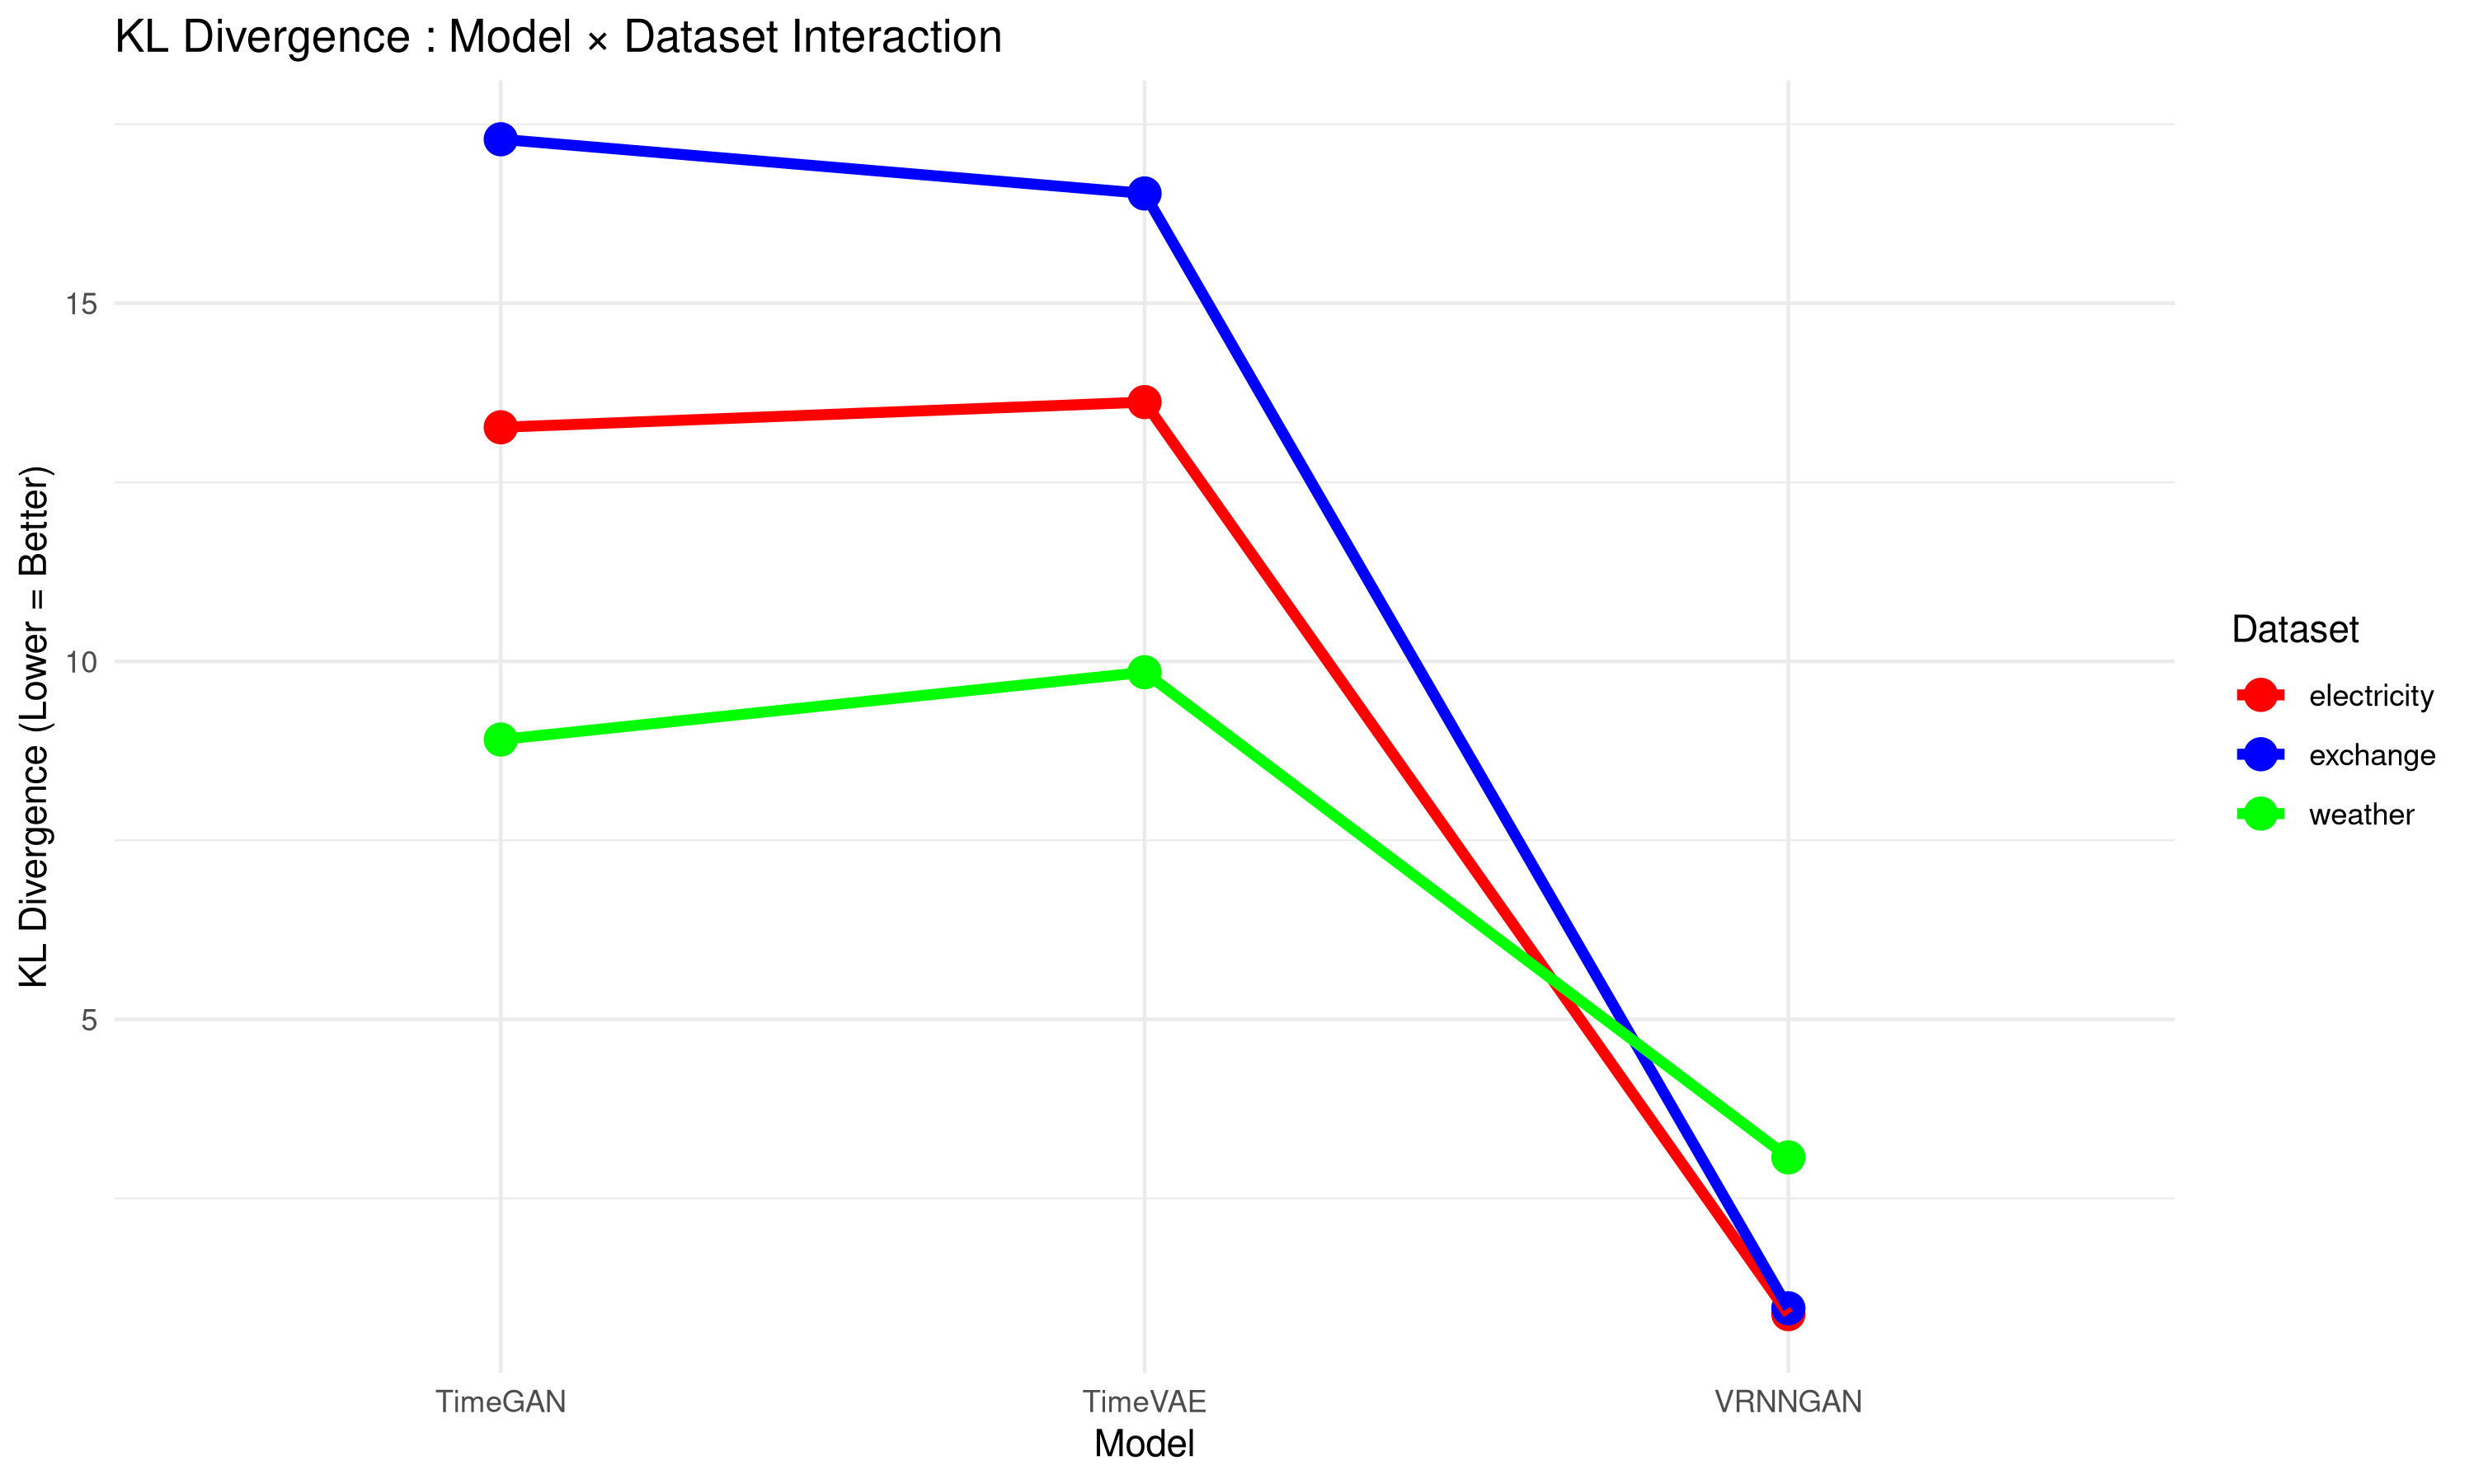
\includegraphics[width=0.8\textwidth]{assets/interaction_kl.png}
\caption{Model × Dataset Interaction Effects for KL Divergence}
\label{fig:kl_interaction}
\end{figure}

The Wasserstein distance interactions, shown in Figure \ref{fig:wasserstein_interaction}, reveal different patterns where TimeVAE demonstrates superior performance specifically for electricity data, while TimeGAN shows advantages for exchange data. These crossing lines exemplify how geometric similarity preservation varies significantly by dataset characteristics.

\begin{figure}[H]
\centering
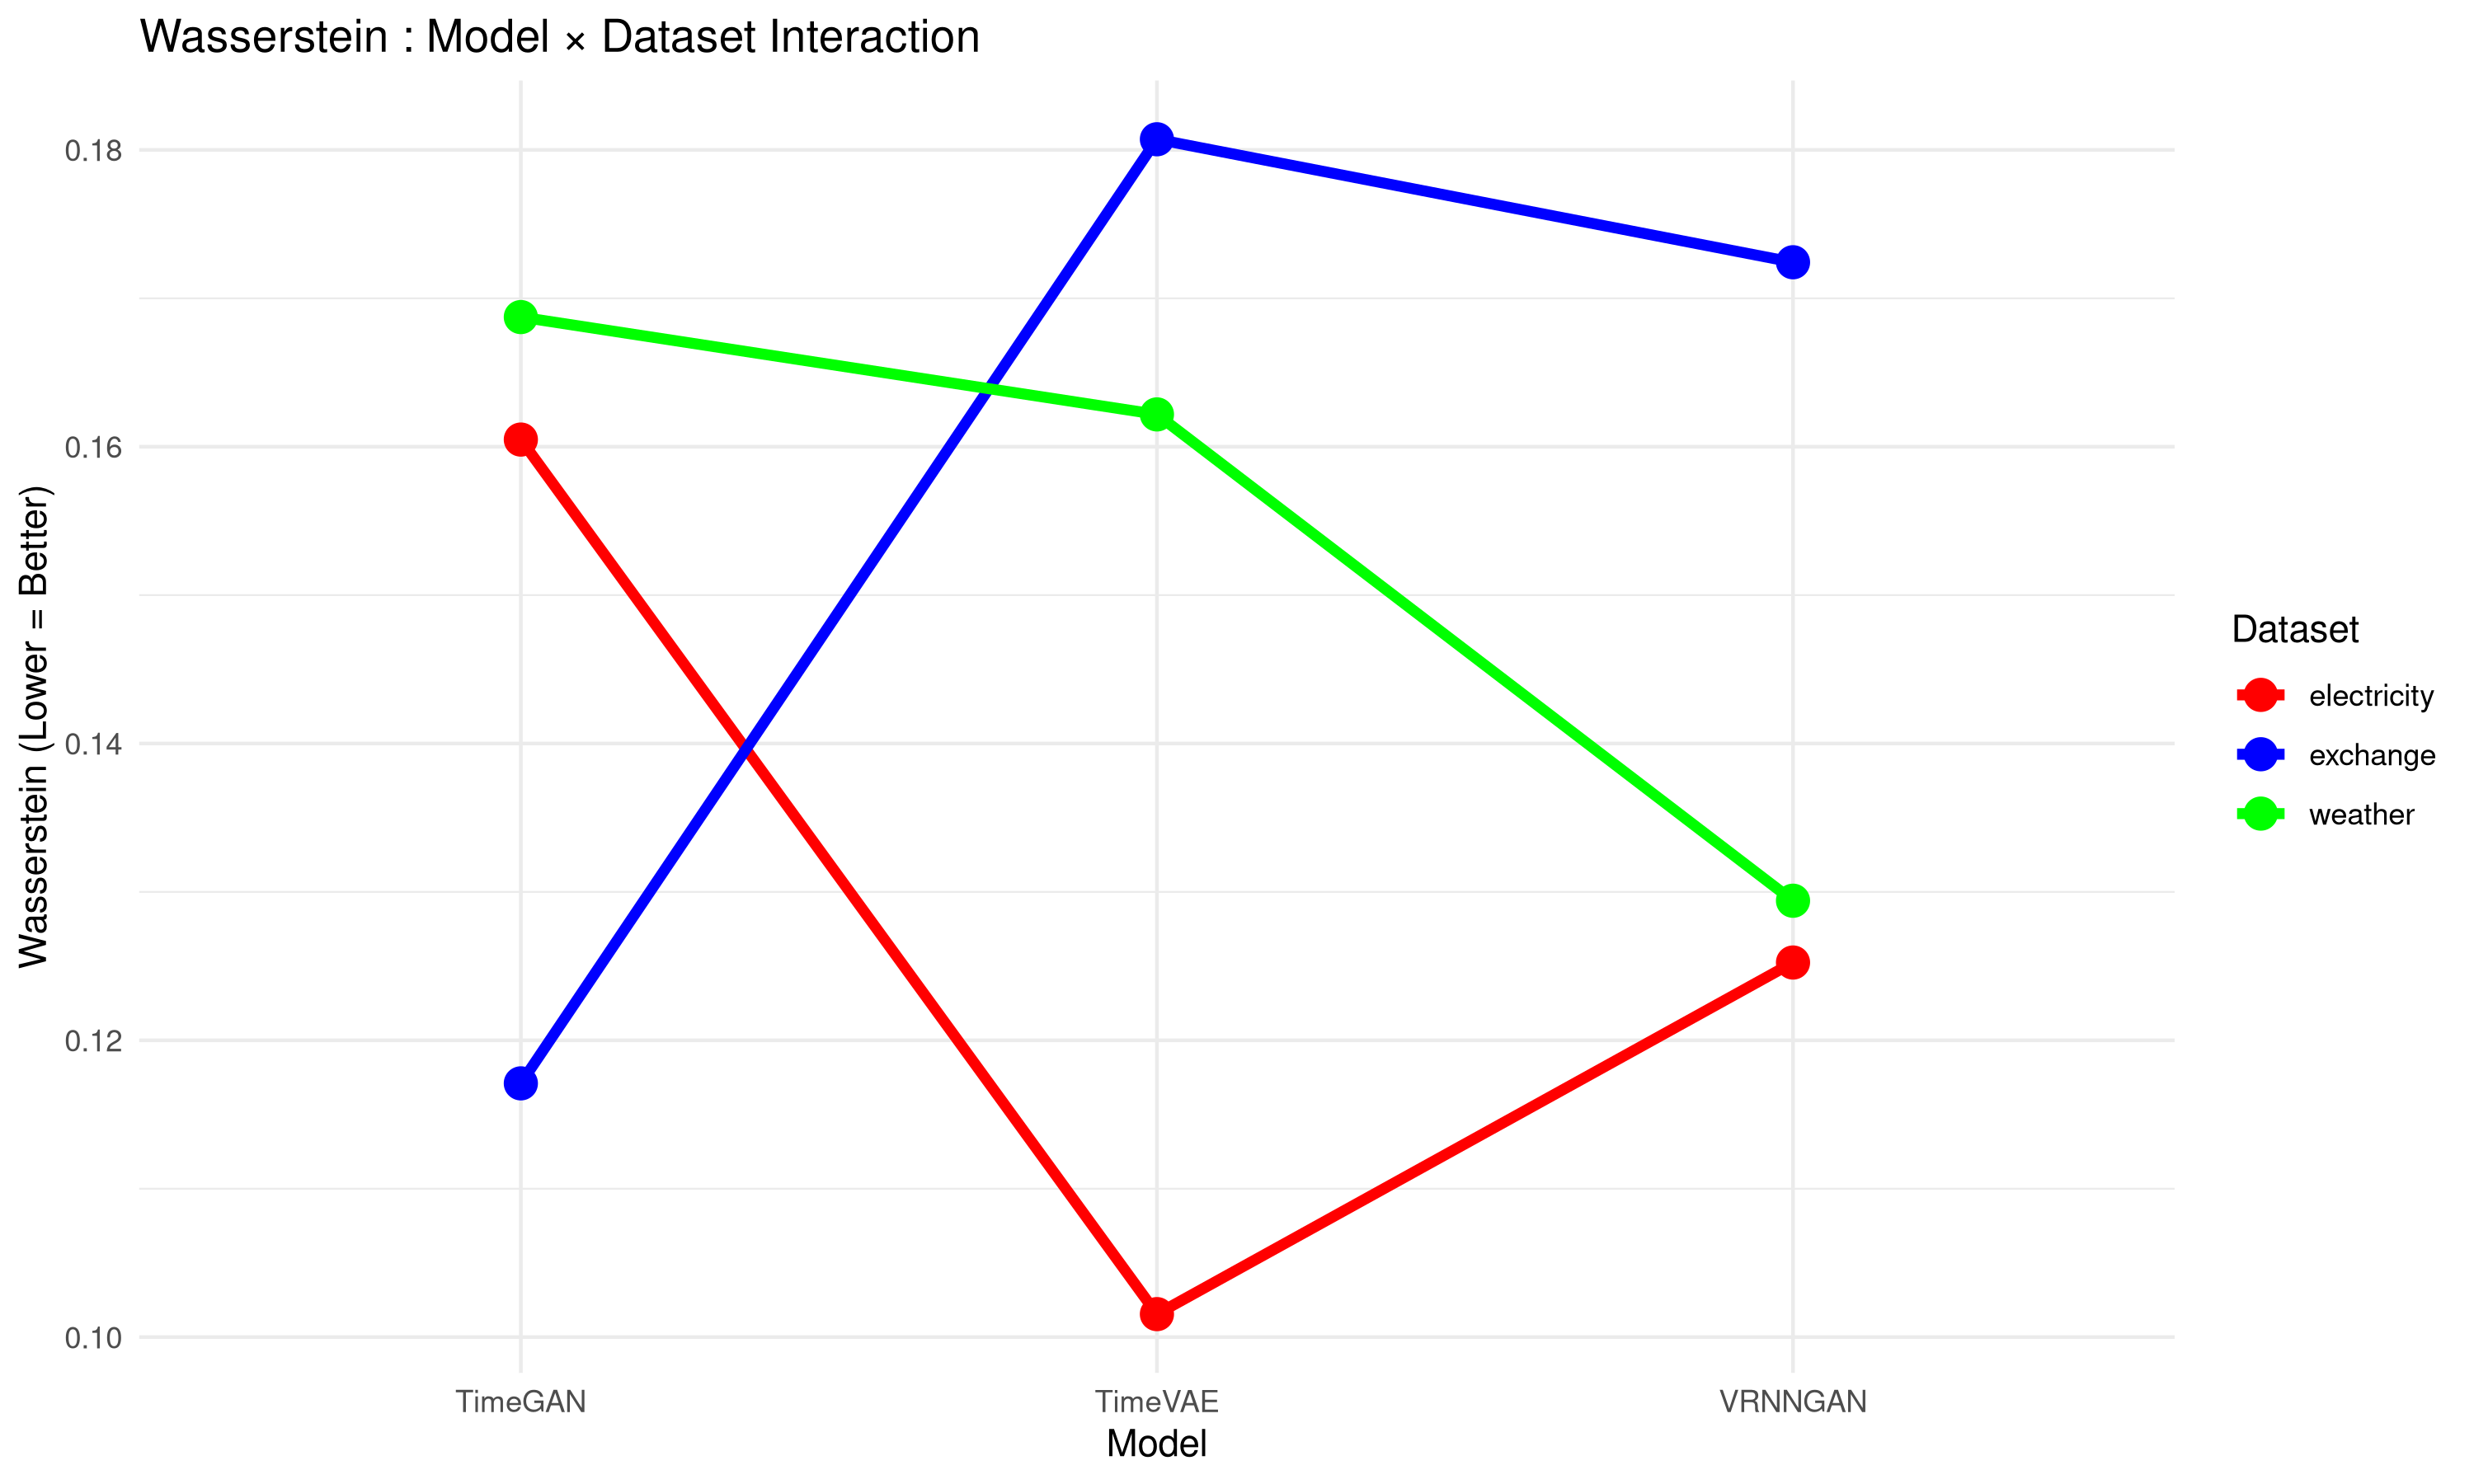
\includegraphics[width=0.8\textwidth]{assets/interaction_wasserstein.png}
\caption{Model × Dataset Interaction Effects for Wasserstein Distance}
\label{fig:wasserstein_interaction}
\end{figure}

Figures \ref{fig:rmse_interaction} and \ref{fig:mae_interaction} display the forecasting performance interactions, where weather data presents unique challenges for all models, particularly affecting TimeVAE performance. The near-parallel lines for electricity and exchange data in both RMSE and MAE suggest more consistent relative model performance for these forecasting metrics across these datasets.

\begin{figure}[H]
\centering
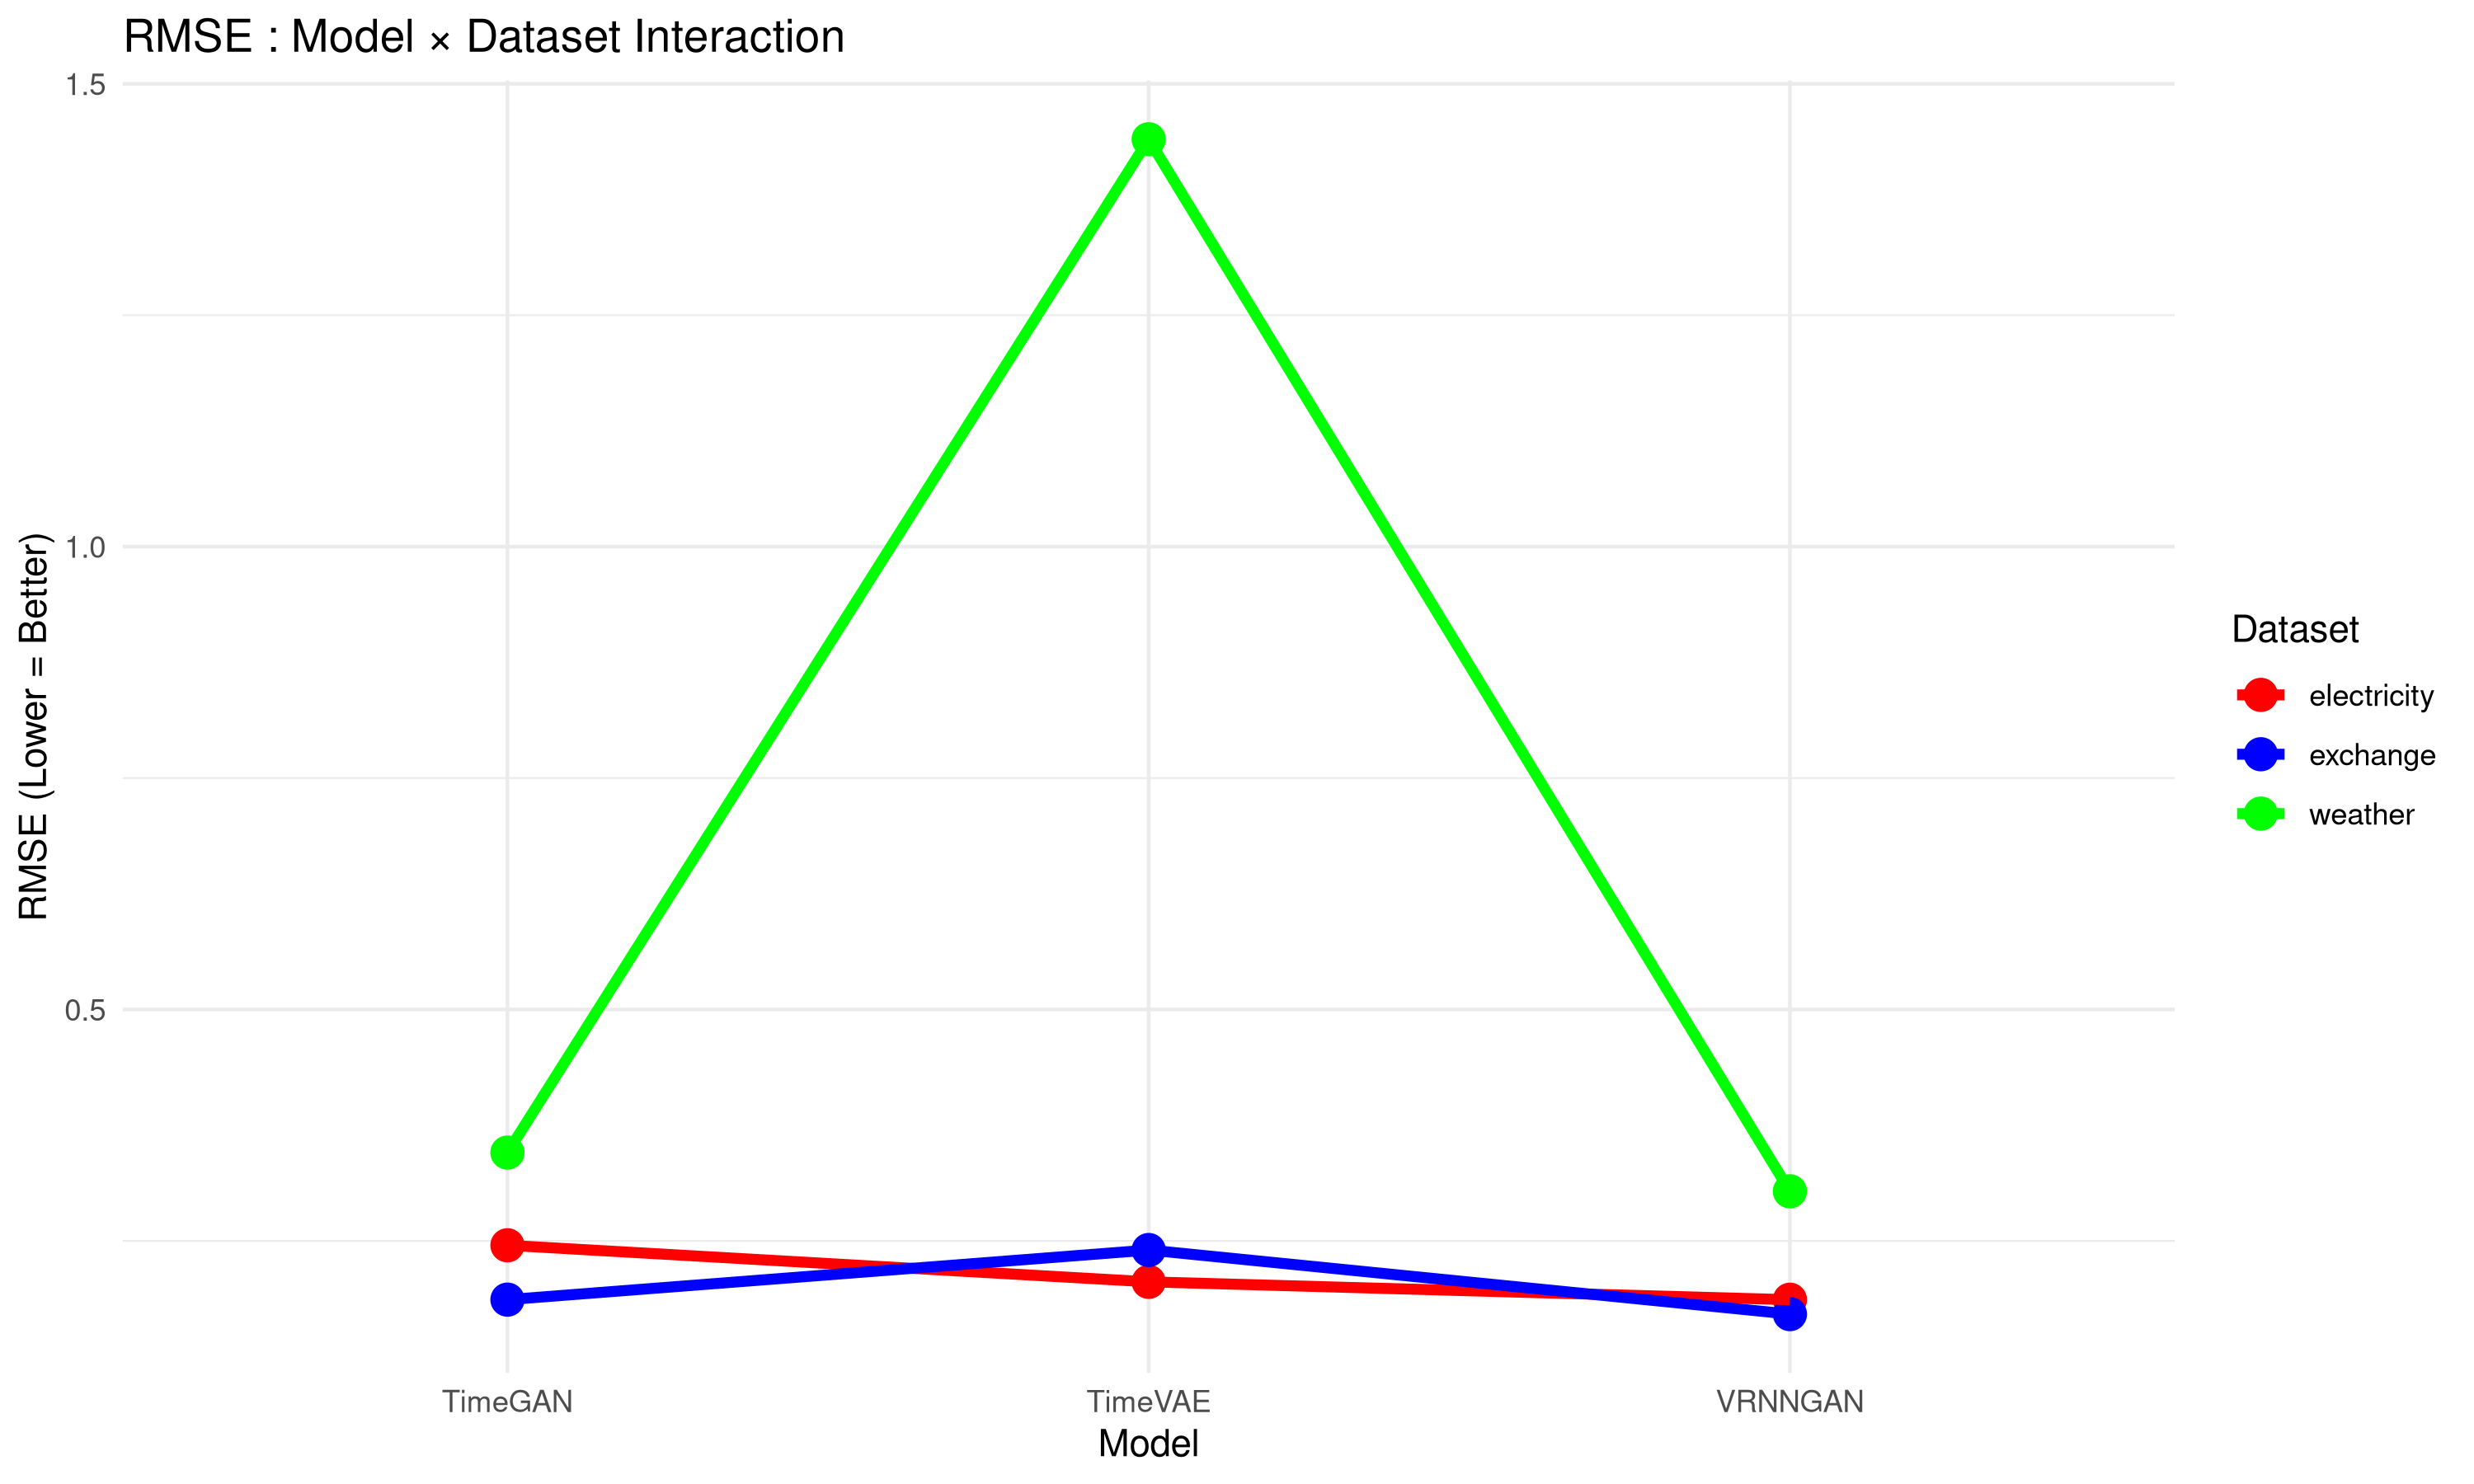
\includegraphics[width=0.8\textwidth]{assets/interaction_rmse.png}
\caption{Model × Dataset Interaction Effects for RMSE}
\label{fig:rmse_interaction}
\end{figure}

\begin{figure}[H]
\centering
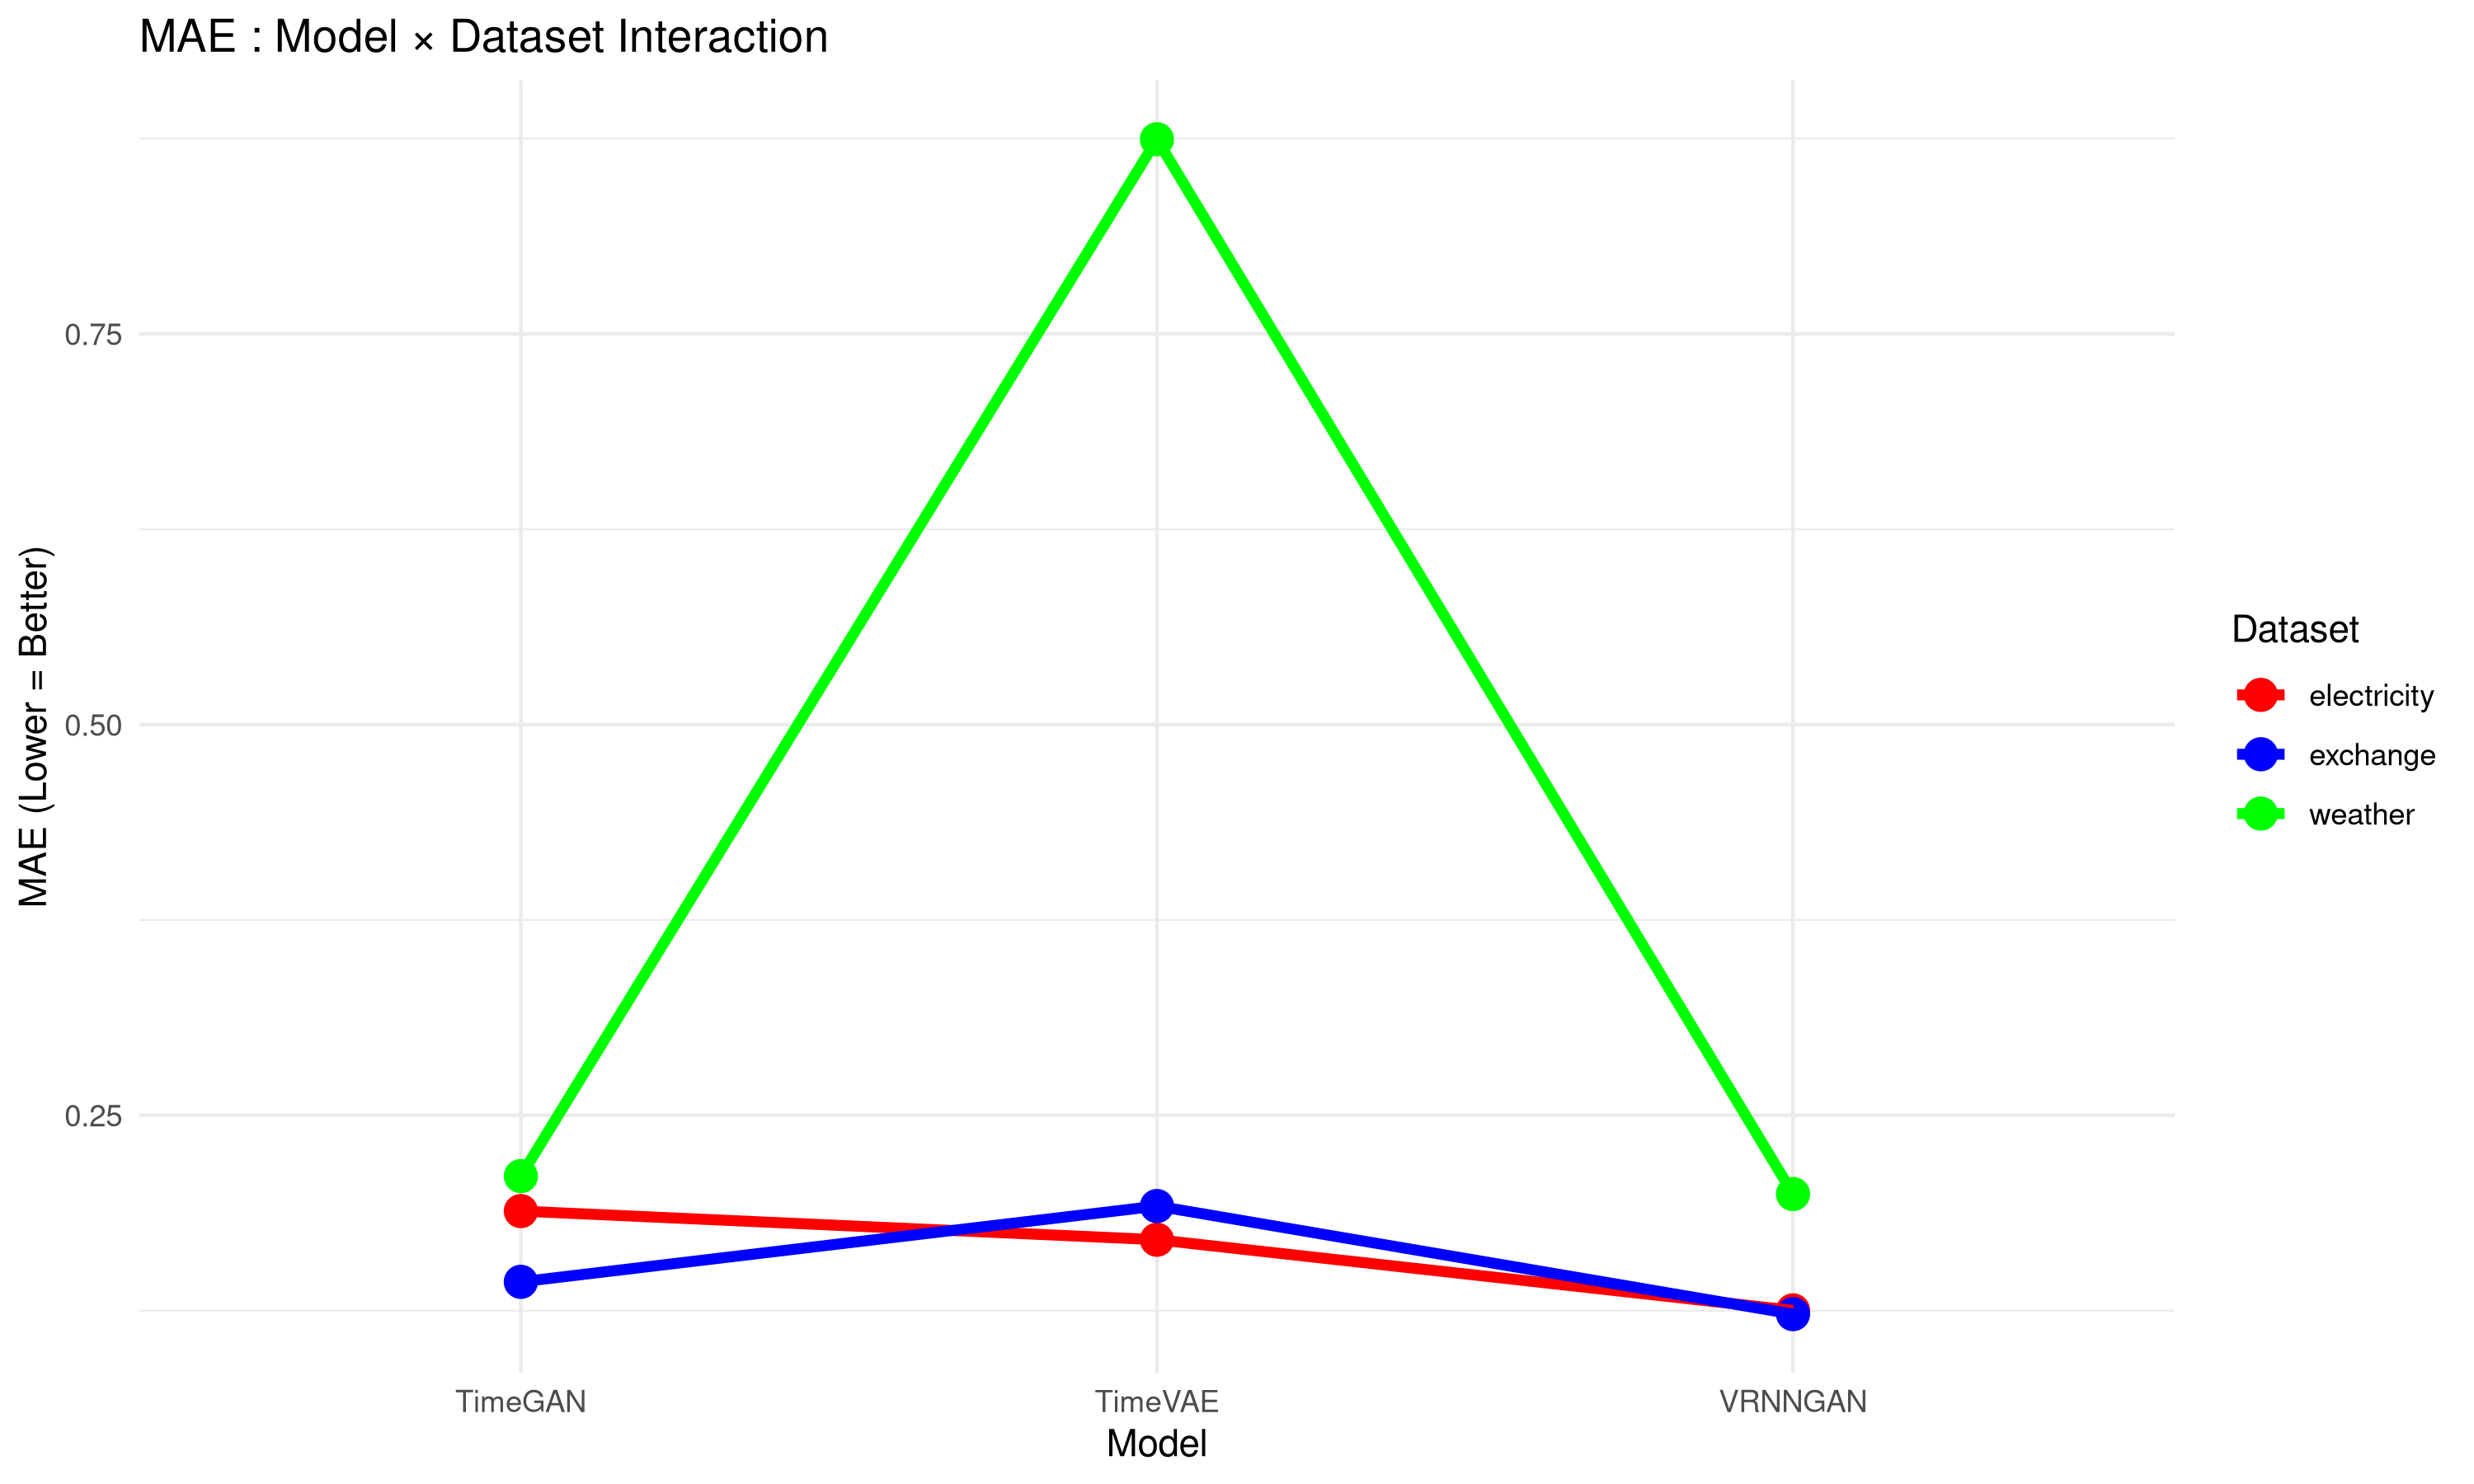
\includegraphics[width=0.8\textwidth]{assets/interaction_mae.png}
\caption{Model × Dataset Interaction Effects for MAE}
\label{fig:mae_interaction}
\end{figure}

These interaction patterns reinforce the ANOVA findings, highlighting that model selection depends on the specific characteristics of the target dataset. The varying interaction strengths across metrics further indicate that different aspects of synthetic data quality, statistical fidelity versus forecasting utility, are affected differently by dataset characteristics. To identify the specific sources of these differences, Tukey HSD post-hoc analysis revealed distinct performance groupings across all metrics, with VRNNGAN consistently forming its own superior performance group while TimeGAN and TimeVAE showed varying relative positions depending on the evaluation context. These statistical foundations necessitate the dataset-specific Shapley analysis that follows to provide interpretable attribution of each model's contribution to synthetic data quality.

\subsubsection{Tukey-HSD Post-Hoc Results}

A closer examination of the post-hoc results illustrates these performance groupings in more detail. For KL divergence results in Table \ref{tab:tukey_kl}, VRNNGAN demonstrates substantially superior performance with a mean value of 1.64, forming its own distinct group (c). TimeGAN and TimeVAE show relatively similar but significantly different performance levels, with TimeGAN (13.16, group a) slightly outperforming TimeVAE (13.33, group b). This pattern indicates that while both individual models struggle with statistical fidelity compared to the hybrid approach, TimeGAN maintains marginally better distributional similarity to the real reference data.

% KL Divergence Tukey HSD Results
\begin{table}[H]
\centering
\caption{Tukey HSD post-hoc analysis for KL divergence}
\label{tab:tukey_kl}
\begin{tabular}{lcc}
\toprule
\textbf{Model} & \textbf{Mean Value} & \textbf{Tukey Group} \\
\midrule
VRNNGAN & 1.6399 & c \\
TimeGAN & 13.1554 & a \\
TimeVAE & 13.3337 & b \\
\bottomrule
\end{tabular}
\footnotesize
\end{table}

The Wasserstein distance results in Table \ref{tab:tukey_wasserstein} reveal a different performance ranking, where all three models form distinct statistical groups despite relatively small absolute differences. VRNNGAN again achieves the best performance (0.142, group c), followed by TimeVAE (0.148, group b) and TimeGAN (0.149, group a). The closer clustering of values suggests that geometric similarity preservation shows less dramatic differences between models compared to statistical divergence measures.

% Wasserstein Distance Tukey HSD Results
\begin{table}[H]
\centering
\caption{Tukey HSD post-hoc analysis for Wasserstein distance}
\label{tab:tukey_wasserstein}
\begin{tabular}{lcc}
\toprule
\textbf{Model} & \textbf{Mean Value} & \textbf{Tukey Group} \\
\midrule
VRNNGAN & 0.1424 & c \\
TimeVAE & 0.1481 & b \\
TimeGAN & 0.1488 & a \\
\bottomrule
\end{tabular}
\footnotesize
\end{table}

For forecasting performance metrics, the post-hoc analysis demonstrates more pronounced differences between models. In RMSE evaluation (Table \ref{tab:tukey_rmse}), VRNNGAN maintains its superior performance (0.220, group c), while TimeGAN (0.259, group a) significantly outperforms TimeVAE (0.629, group b). This notable gap indicates that TimeVAE's approach to latent space modeling may not effectively capture the temporal dependencies necessary for accurate forecasting. Similarly, MAE results (Table \ref{tab:tukey_mae}) confirm this pattern, with VRNNGAN (0.149, group c) leading, followed by TimeGAN (0.181, group a), and TimeVAE showing notably higher error rates (0.412, group b).


% RMSE Tukey HSD Results
\begin{table}[H]
\centering
\caption{Tukey HSD post-hoc analysis for RMSE}
\label{tab:tukey_rmse}
\begin{tabular}{lcc}
\toprule
\textbf{Model} & \textbf{Mean Value} & \textbf{Tukey Group} \\
\midrule
VRNNGAN & 0.2203 & c \\
TimeGAN & 0.2591 & a \\
TimeVAE & 0.6287 & b \\
\bottomrule
\end{tabular}
\footnotesize
\end{table}

% MAE Tukey HSD Results
\begin{table}[H]
\centering
\caption{Tukey HSD post-hoc analysis for MAE}
\label{tab:tukey_mae}
\begin{tabular}{lcc}
\toprule
\textbf{Model} & \textbf{Mean Value} & \textbf{Tukey Group} \\
\midrule
VRNNGAN & 0.1492 & c \\
TimeGAN & 0.1811 & a \\
TimeVAE & 0.4123 & b \\
\bottomrule
\end{tabular}
\footnotesize
\end{table}

The consistent emergence of three distinct statistical groups across all metrics confirms that each model contributes unique characteristics to synthetic data generation. VRNNGAN's consistent placement in the superior performance group (c) across all metrics validates the effectiveness of hybrid architectures in balancing multiple aspects of data quality. The varying relative positions of TimeGAN and TimeVAE across different metrics highlight the trade-offs inherent in different generative approaches, with TimeGAN showing particular strength in forecasting tasks and TimeVAE demonstrating competitive performance in certain geometric similarity measures.

\subsection{Shapley Value Analysis}
The Shapley analysis reveals the individual contributions of each model component to the overall performance across different metrics and datasets. For each metric evaluated, the analysis examines the marginal contributions and interactions between model components.

\subsubsection{Cross-Metric Performance Patterns}

Figures~\ref{fig:shapley_kl} through~\ref{fig:shapley_mae} present the Shapley value contributions of each generative model across all datasets for each evaluation metric. This cross-metric perspective reveals how architectural approaches contribute to specific aspects of synthetic data quality, independent of dataset characteristics.

KL divergence analysis (Figure~\ref{fig:shapley_kl}) demonstrates VRNNGAN's consistent superiority in statistical fidelity preservation across all temporal contexts. The hybrid architecture maintains positive contributions regardless of dataset complexity, while TimeGAN and TimeVAE exhibit context-dependent performance with substantially lower overall contributions.

\begin{figure}[H]
\centering
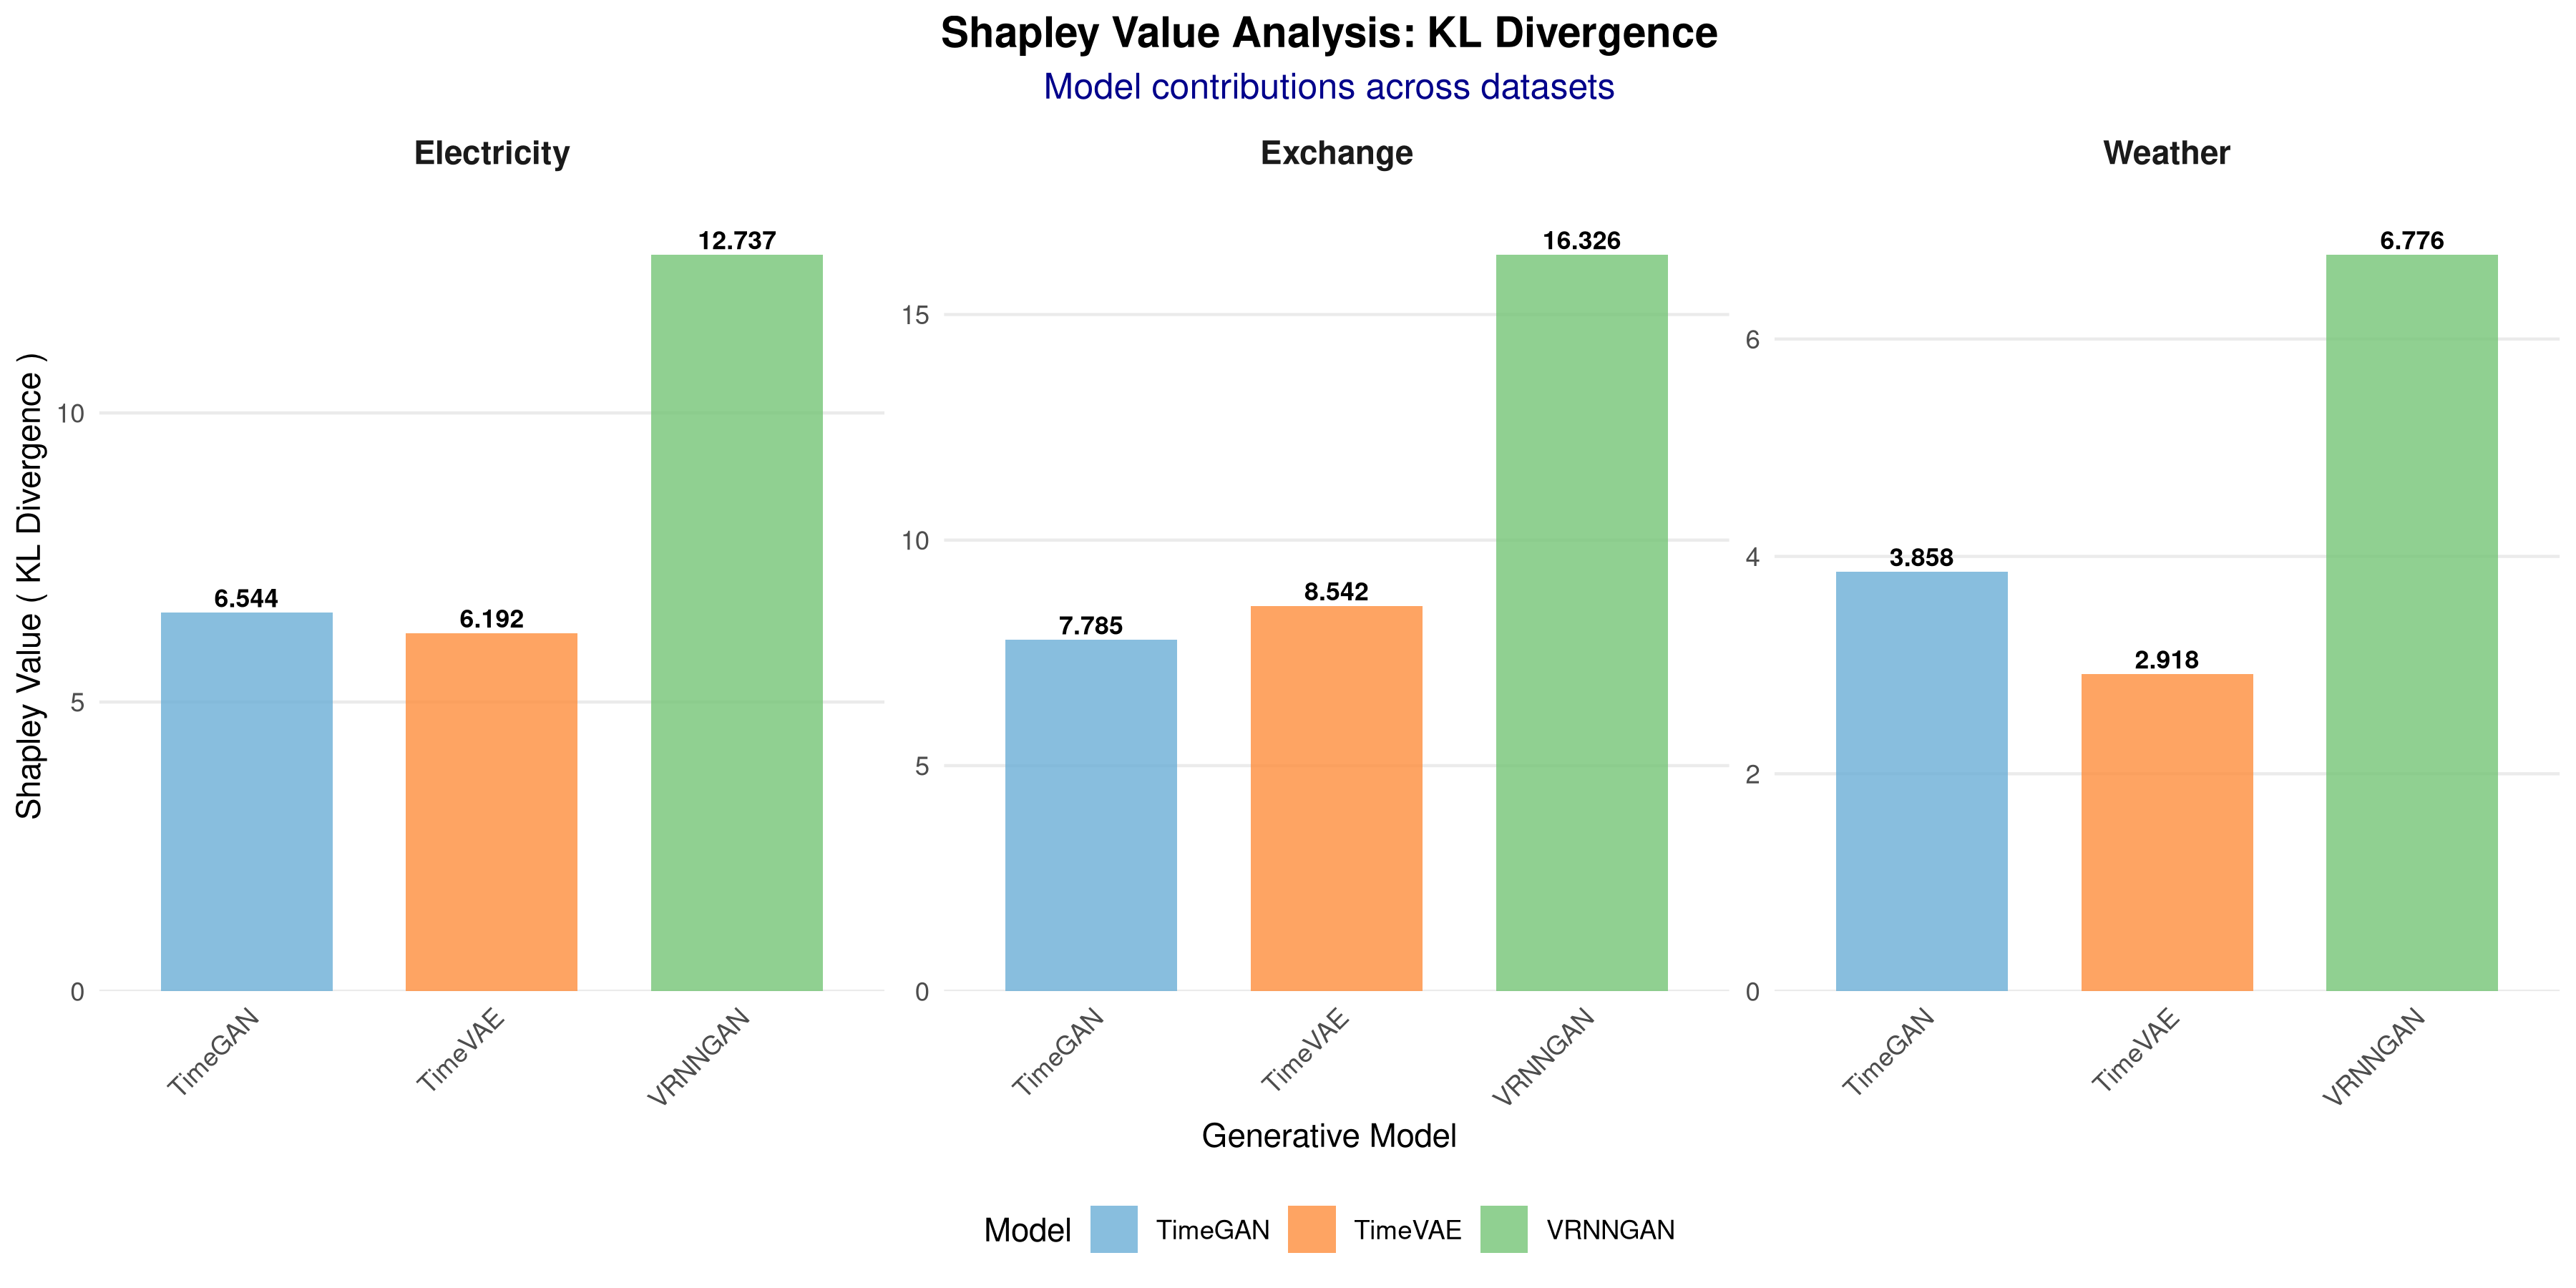
\includegraphics[width=0.8\textwidth]{assets/shapley_kl_analysis.png}
\caption{Shapley Value Analysis for KL Divergence across Models and Datasets}
\label{fig:shapley_kl}
\end{figure}

Wasserstein distance patterns (Figure~\ref{fig:shapley_wasserstein}) reveal the most pronounced context sensitivity among all metrics. Unlike statistical fidelity where VRNNGAN demonstrates universal advantages, geometric similarity preservation shows no single architectural winner. Each model demonstrates dataset-specific strengths, with negative Shapley values emerging for certain combinations, indicating fundamental incompatibilities between specific architectures and temporal pattern types.

\begin{figure}[H]
\centering
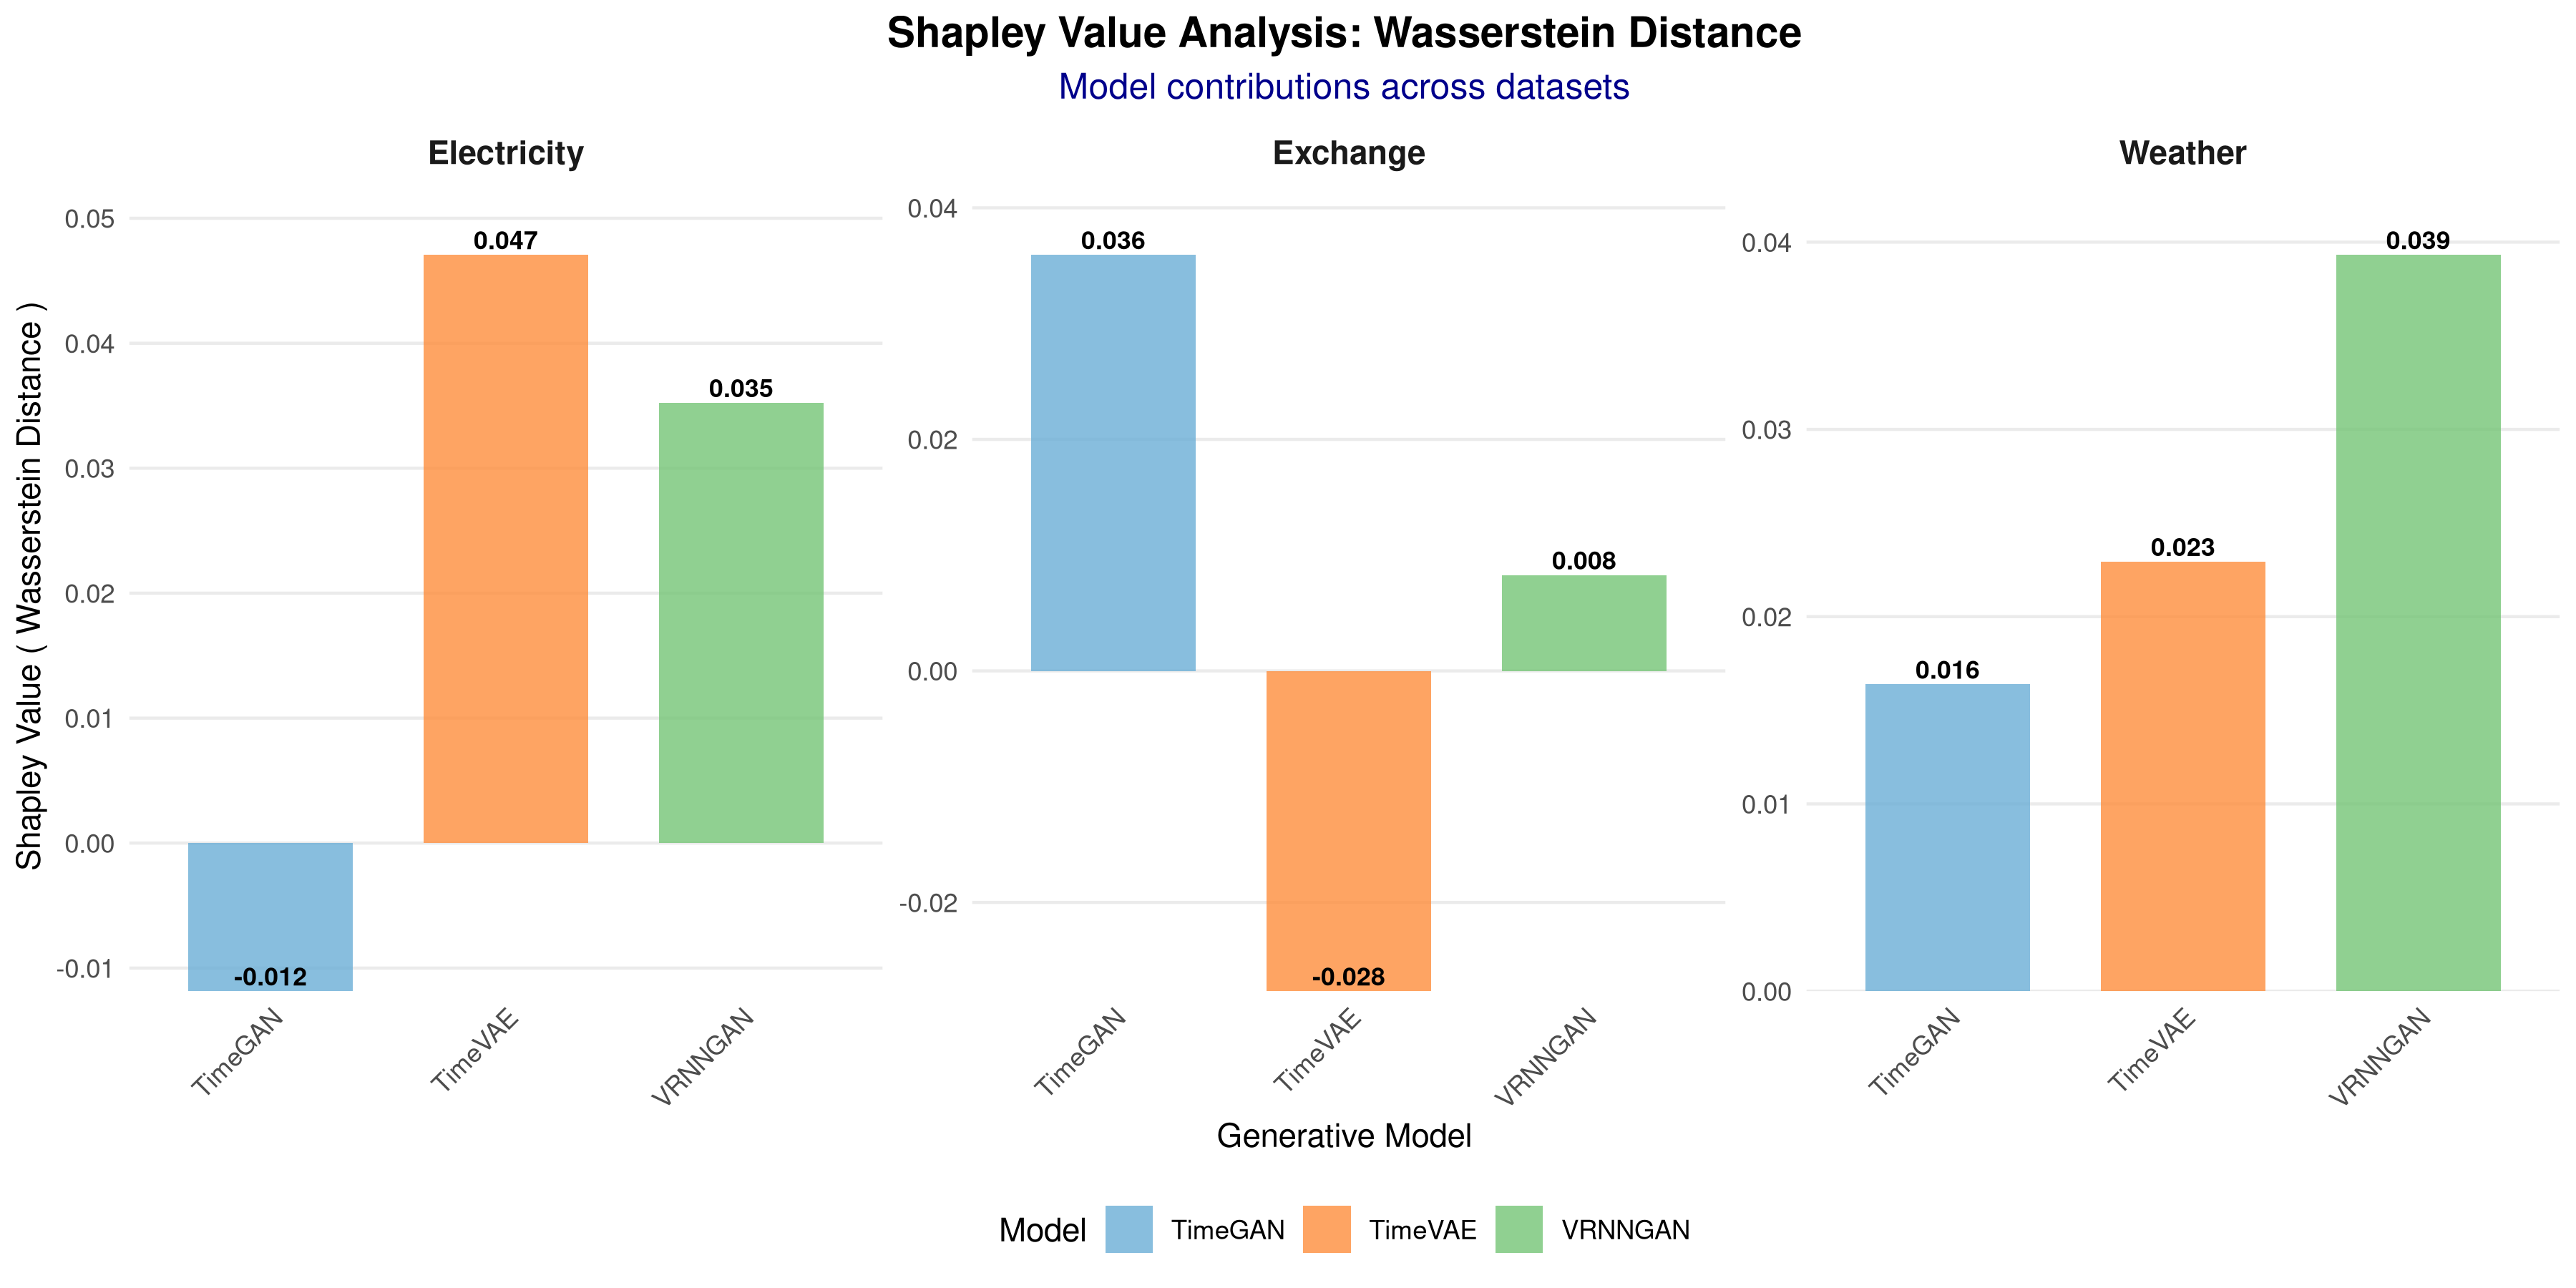
\includegraphics[width=0.8\textwidth]{assets/shapley_wasserstein_analysis.png}
\caption{Shapley Value Analysis for Wasserstein Distance across Models and Datasets}
\label{fig:shapley_wasserstein}
\end{figure}

Forecasting utility metrics exhibit consistent patterns across both RMSE (Figure~\ref{fig:shapley_rmse}) and MAE (Figure~\ref{fig:shapley_mae}). VRNNGAN maintains the highest contributions across all datasets, reinforcing its effectiveness in preserving temporal dependencies necessary for downstream prediction tasks. TimeVAE demonstrates substantially reduced forecasting contributions, particularly for weather and exchange datasets, while TimeGAN shows moderate contribution levels across most contexts.
\begin{figure}[H]
\centering
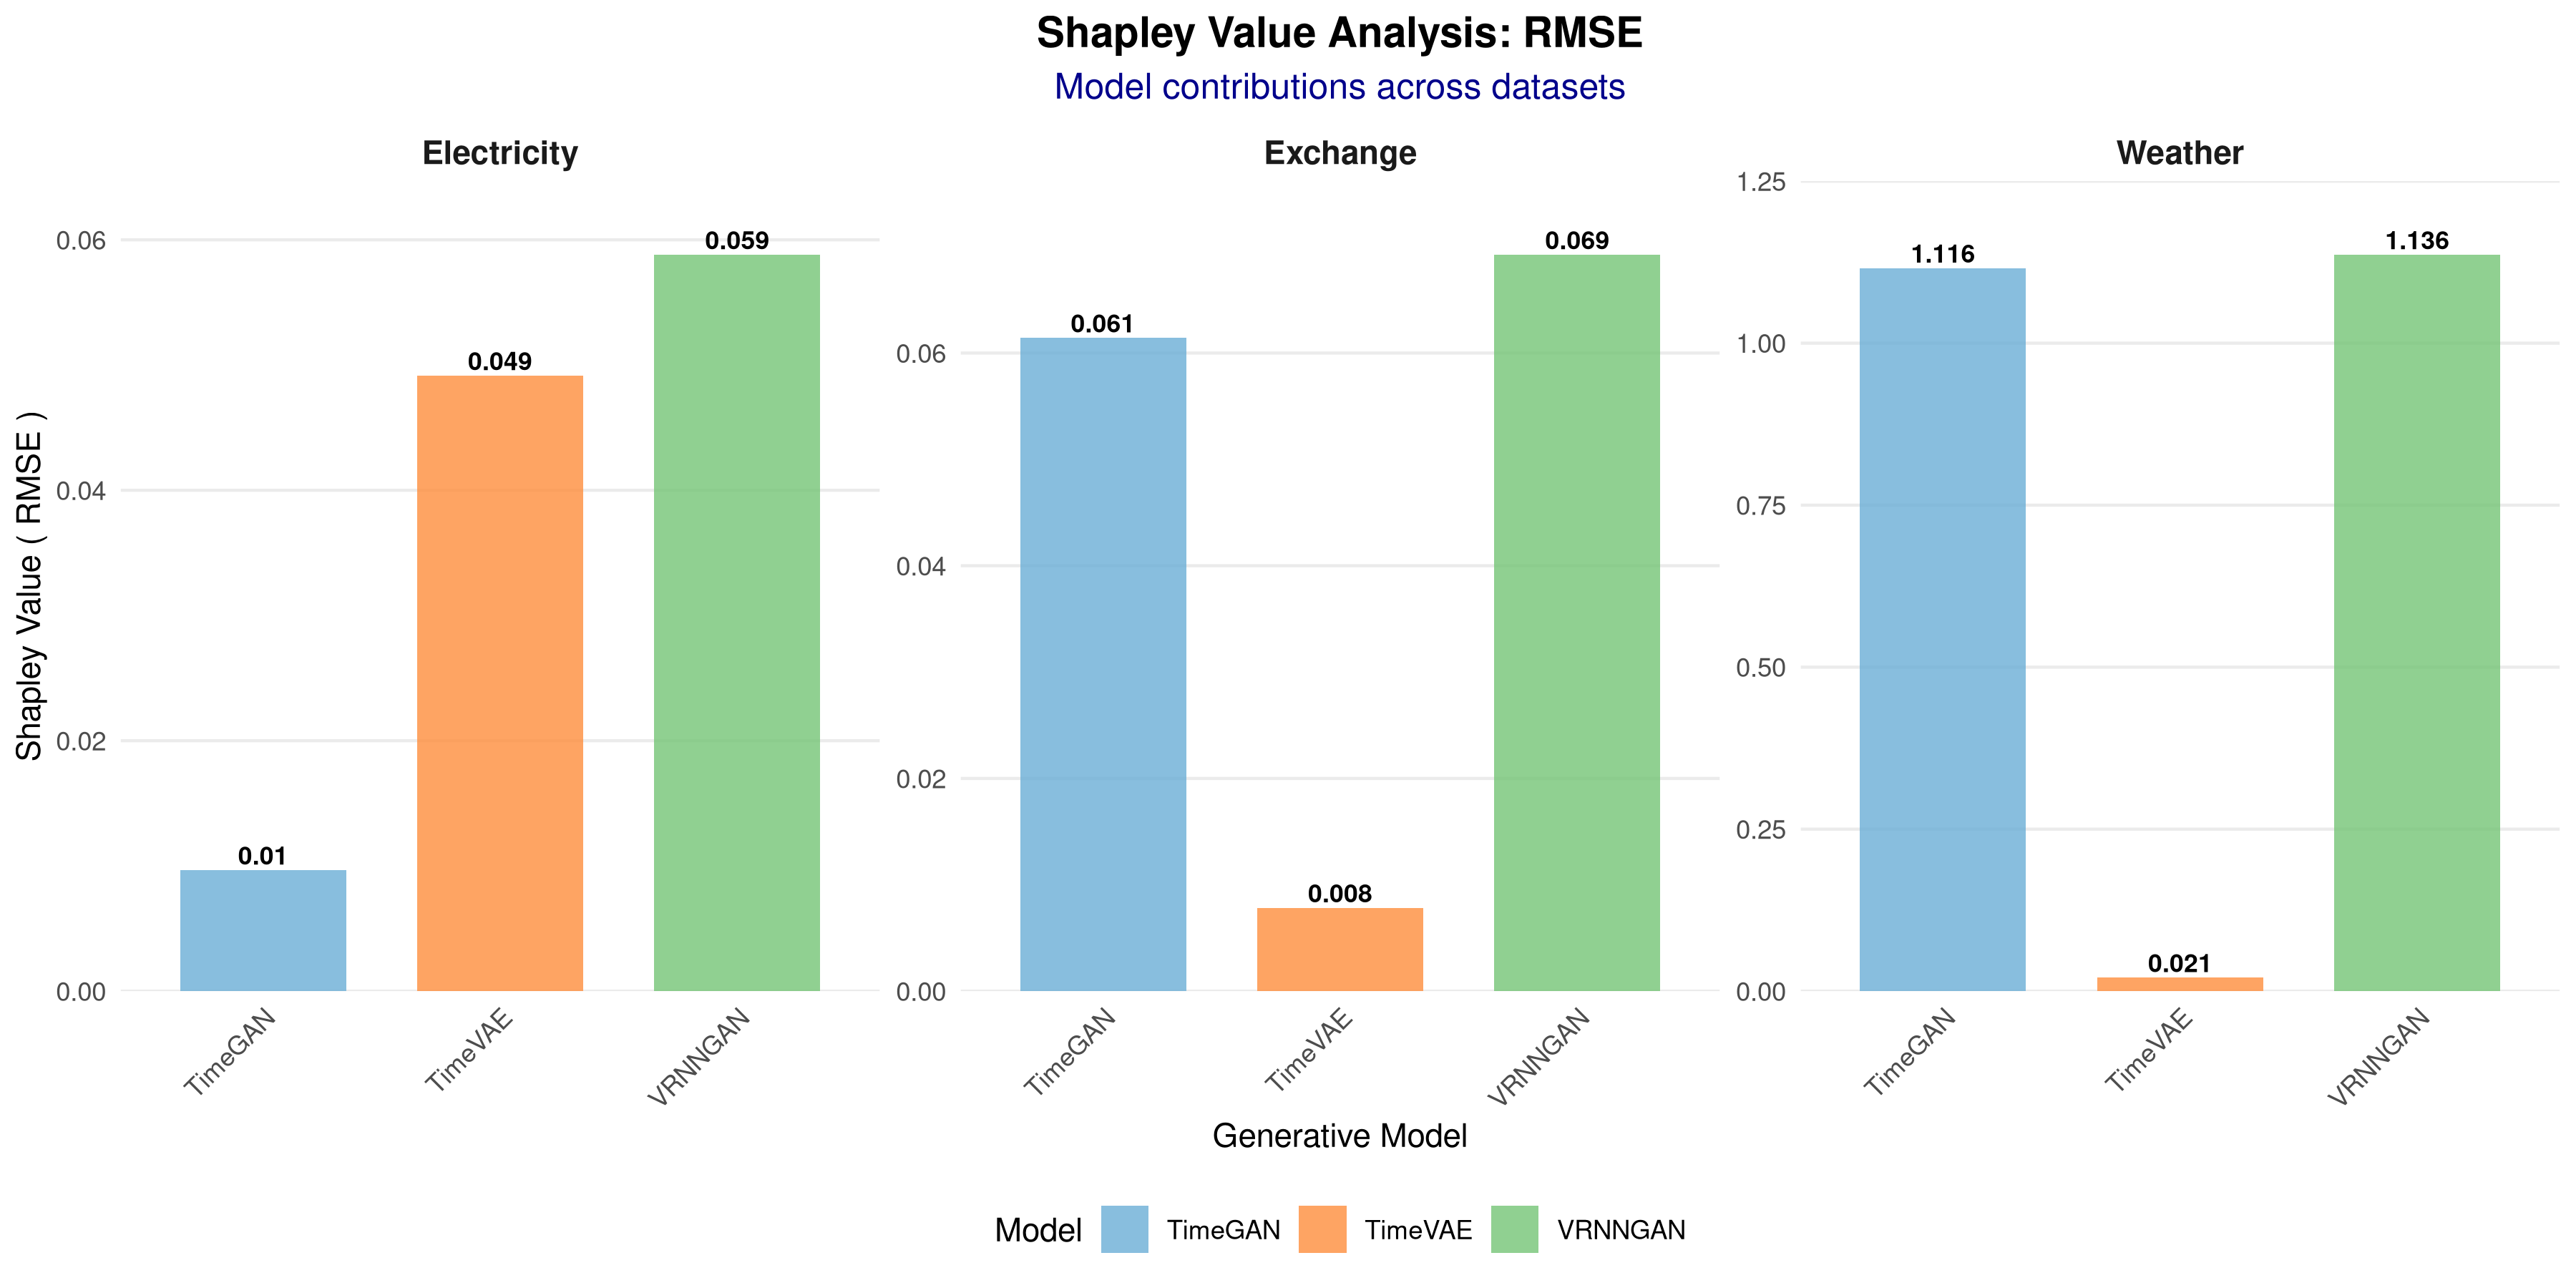
\includegraphics[width=0.8\textwidth]{assets/shapley_rmse_analysis.png}
\caption{Shapley Value Analysis for RMSE across Models and Datasets}
\label{fig:shapley_rmse}
\end{figure}

\begin{figure}[H]
\centering
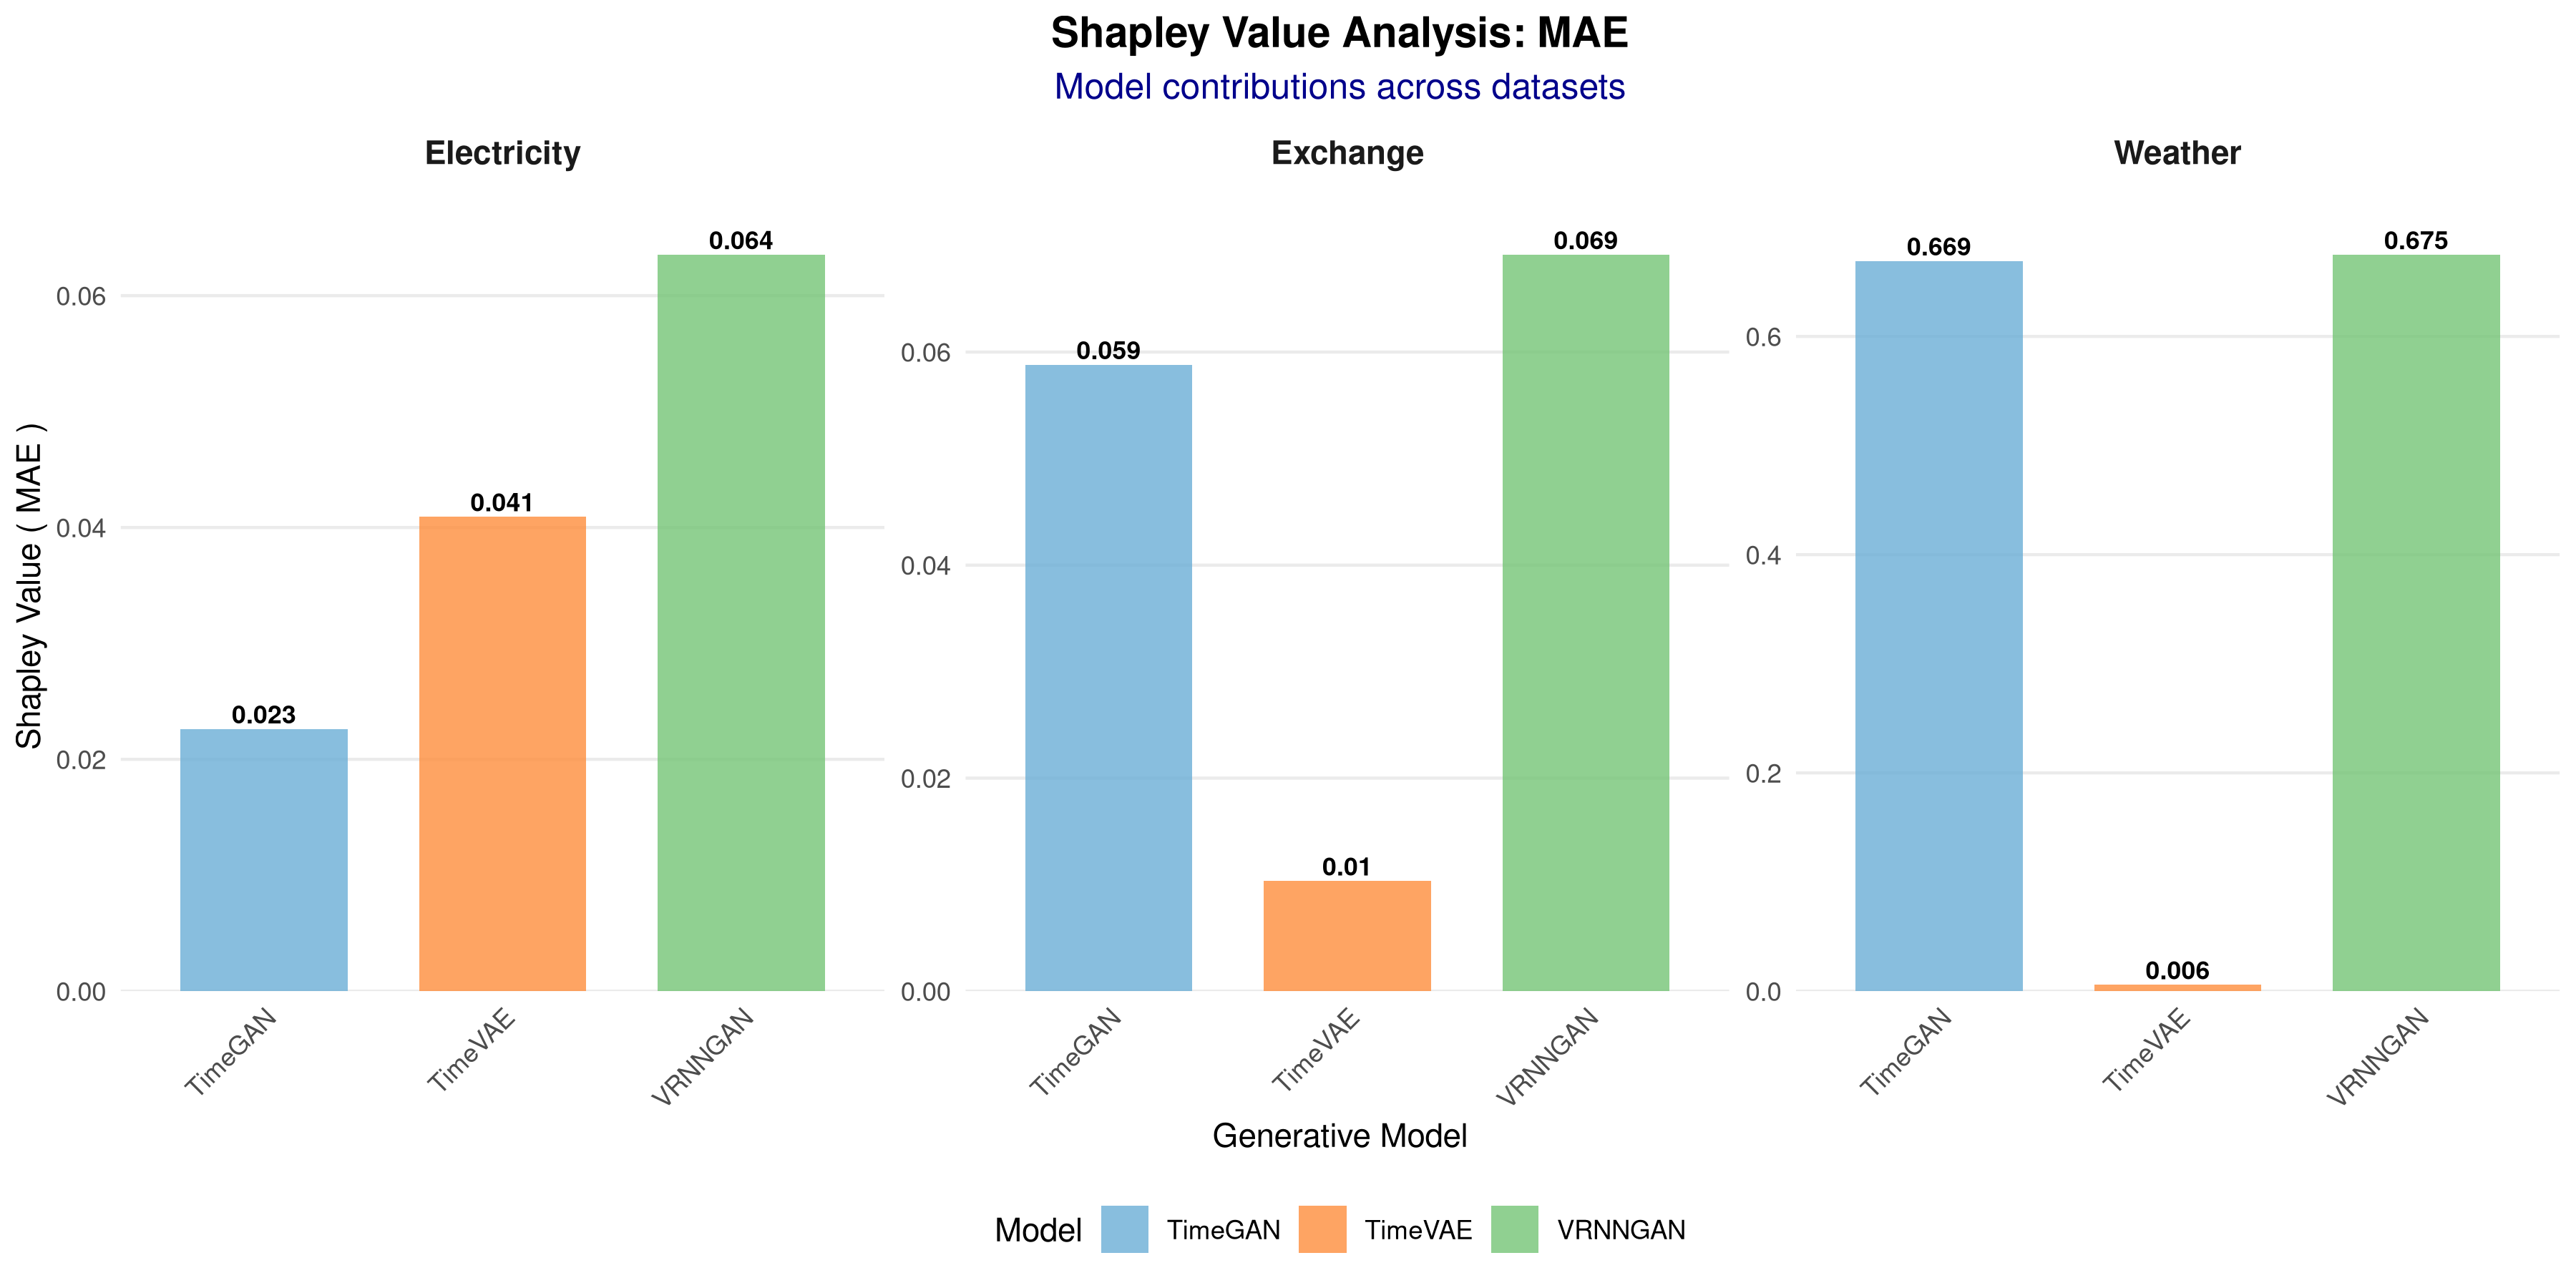
\includegraphics[width=0.8\textwidth]{assets/shapley_mae_analysis.png}
\caption{Shapley Value Analysis for MAE across Models and Datasets}
\label{fig:shapley_mae}
\end{figure}

These cross-metric patterns establish the fundamental behavioral differences between architectural approaches, revealing that hybrid models provide consistent advantages for statistical fidelity and forecasting utility, while geometric similarity preservation remains highly context-dependent. The following analysis examines specific dataset characteristics to understand what drives these observed performance variations.

\subsubsection{Dataset-Specific Performance Attribution}

Each dataset presents unique temporal characteristics that favor different architectural approaches, revealing the underlying factors that determine optimal model selection for specific data contexts.

The electricity dataset's regular load patterns create unique evaluation challenges that favor different architectural approaches depending on the quality dimension assessed. Table~\ref{tab:shapley_electricity} reveals that VRNNGAN dominates statistical fidelity (KL: 12.737) and forecasting metrics (RMSE: 0.059, MAE: 0.064), demonstrating the hybrid architecture's effectiveness for structured temporal dependencies. However, TimeVAE's superior Wasserstein performance (0.047) indicates that variational approaches excel at preserving geometric similarities in regular, predictable patterns where smooth latent space interpolation aligns with underlying data structure. TimeGAN's negative Wasserstein contribution (-0.012) suggests that adversarial training may introduce artifacts that distort geometric relationships in highly structured temporal data.


\begin{table}[H]
\centering
\caption{Shapley value contributions for the electricity dataset}
\label{tab:shapley_electricity}
\begin{tabular}{lcccc}
\toprule
\textbf{Approach} & \textbf{KL Divergence} & \textbf{Wasserstein} & \textbf{RMSE} & \textbf{MAE} \\
\midrule
TimeGAN & 6.544 & -0.012 & 0.010 & 0.023 \\
TimeVAE & 6.193 & \textbf{0.047} & 0.050 & 0.041 \\
VRNNGAN & \textbf{12.737} & 0.035 & \textbf{0.059} & \textbf{0.064} \\
\bottomrule
\end{tabular}
\\[0.5em]
\footnotesize
\textit{Note: Bold indicates highest Shapley value (best contributor) per metric.}
\end{table}

Financial time series characteristics present distinct challenges that reveal complementary strengths across architectural paradigms. Table~\ref{tab:shapley_exchange} shows VRNNGAN achieving exceptional statistical fidelity (KL: 16.326), the highest observed across all experiments, indicating superior distributional modeling for volatile financial patterns. TimeGAN's Wasserstein advantage (0.036) demonstrates that adversarial training effectively captures the stochastic nature of exchange rate fluctuations, while TimeVAE's negative contribution (-0.028) reveals fundamental limitations in variational approaches for modeling financial volatility. These patterns suggest that financial data complexity requires either sophisticated hybrid architectures or adversarial approaches specifically designed for non-stationary temporal patterns.

\begin{table}[H]
\centering
\caption{Shapley value contributions for the exchange dataset}
\label{tab:shapley_exchange}
\begin{tabular}{lcccc}
\toprule
\textbf{Approach} & \textbf{KL Divergence} & \textbf{Wasserstein} & \textbf{RMSE} & \textbf{MAE} \\
\midrule
TimeGAN & 7.785 & \textbf{0.036} & 0.061 & 0.059 \\
TimeVAE & 8.542 & -0.028 & 0.008 & 0.010 \\
VRNNGAN & \textbf{16.326} & 0.008 & \textbf{0.069} & \textbf{0.069} \\
\bottomrule
\end{tabular}
\\[0.5em]
\footnotesize
\textit{Note: Bold indicates highest Shapley value (best contributor) per metric.}
\end{table}

Weather data presents the most challenging evaluation context, with VRNNGAN demonstrating consistent superiority across all metrics while individual models show substantial performance variations. Table~\ref{tab:shapley_weather} confirms VRNNGAN's robust performance (KL: 6.776, Wasserstein: 0.039, RMSE: 1.137, MAE: 0.675), highlighting how meteorological complexity requires sophisticated architectural combinations to maintain synthetic data quality. The substantial Shapley value ranges across models reflect the inherent difficulty of capturing meteorological relationships, where seasonal patterns, non-linear dependencies, and multi-scale temporal interactions challenge individual generative approaches.

\begin{table}[H]
\centering
\caption{Shapley value contributions for the weather dataset}
\label{tab:shapley_weather}
\begin{tabular}{lcccc}
\toprule
\textbf{Approach} & \textbf{KL Divergence} & \textbf{Wasserstein} & \textbf{RMSE} & \textbf{MAE} \\
\midrule
TimeGAN & 3.858 & 0.016 & 1.116 & 0.669 \\
TimeVAE & 2.918 & 0.023 & 0.21 & 0.006 \\
VRNNGAN & \textbf{6.776} & \textbf{0.039} & \textbf{1.137} & \textbf{0.675} \\
\bottomrule
\end{tabular}
\\[0.5em]
\footnotesize
\textit{Note: Bold indicates highest Shapley value (best contributor) per metric.}
\end{table}

\subsection{Discussion}

The statistical analysis reveals a coherent pattern of findings that illuminate both the individual strengths of generative models and their complex interactions with dataset characteristics. The significant main effects identified through ANOVA (all F-statistics $>$ 100, p $<$ 0.001) combined with the Tukey HSD post-hoc results establish VRNNGAN's consistent superiority across evaluation metrics, while the substantial Model × Dataset interactions demonstrate that synthetic data generation effectiveness is fundamentally context-dependent rather than universal.

\subsubsection*{Hybrid Architecture Synergy and Performance Patterns}

This statistical foundation provides empirical support for the Shapley value analysis, which reveals that VRNNGAN's advantages stem from genuine architectural synergy rather than merely additive benefits of combining VAE and GAN approaches. The hybrid model's KL divergence Shapley values ranging from 6.776 to 16.326 compared to individual models' contributions of 2.918 to 8.542 demonstrate significant improvements in statistical fidelity preservation. Similarly, VRNNGAN consistently achieves the highest Shapley values for forecasting utility metrics, with RMSE contributions ranging from 0.059 to 1.137 and MAE contributions from 0.064 to 0.675, confirming enhanced practical utility across all datasets.

The consistent superiority of the hybrid architecture extends beyond the comparative advantages identified in previous literature. While \textcite{yoon_time-series_2019} focused on demonstrating TimeGAN's effectiveness against other GAN variants, and \textcite{desai_timevae_2021} showed TimeVAE's competitive performance against TimeGAN in specific contexts, this study provides the first systematic evidence that combining the GAN and VAE approaches yields synergistic benefits. The Shapley analysis framework enables quantification of how GAN and VAE components contribute to overall performance, revealing that VRNNGAN's success stems from architectural complementarity rather than simple performance averaging.

\subsubsection*{Context-Dependent Model Effectiveness}

Notably, while VRNNGAN demonstrates consistent superiority across most evaluation contexts, winning 10 out of 12 metric-dataset combinations in the Shapley analysis, the relative rankings between TimeGAN and TimeVAE are not fixed and vary considerably depending on the evaluation context. This finding reinforces the context-dependent nature of generative model effectiveness and underscores the importance of comprehensive evaluation frameworks rather than relying on single-context comparisons.

Most notably, the Wasserstein distance metric reveals the clearest evidence of context-dependent model effectiveness, with each dataset favoring a different generative approach for geometric similarity preservation. For electricity data, TimeVAE achieves the highest Shapley value (0.047), demonstrating the effectiveness of variational approaches for structured temporal patterns with regular load distributions. In contrast, exchange data favors TimeGAN with the highest Wasserstein Shapley value (0.036), while TimeVAE shows negative contribution (-0.028), indicating that adversarial training better captures the stochastic volatility and irregular patterns characteristic of financial time series. Weather data demonstrates VRNNGAN's superiority (0.039), completing the pattern where each dataset-metric combination reveals distinct architectural advantages.

\subsubsection*{Model Limitations and Negative Contributions}

The emergence of negative Shapley values provides novel insights into model limitations under specific contexts. TimeGAN's negative Wasserstein contribution (-0.012) for electricity data and TimeVAE's negative contribution (-0.028) for exchange data reveal context-specific performance limitations that extend beyond simple underperformance. These negative contributions indicate that certain architectural approaches can actually detract from overall synthetic data quality when applied to incompatible temporal patterns. This represents a fundamental shift from viewing model selection as choosing the best performer to understanding when certain approaches should be explicitly avoided for specific data contexts.

\subsubsection*{Methodological Contributions and Framework Advancement}

The application of Shapley value analysis to generative model evaluation represents a significant methodological advancement that addresses evaluation challenges identified in recent literature reviews by \textcite{goyal_systematic_2024}. The framework successfully provides interpretable attribution of model contributions while maintaining mathematical rigor through fair allocation principles. The bootstrap methodology with 15 iterations per model-dataset combination provided sufficient statistical power for robust evaluation while revealing consistent performance patterns that inform practical model selection decisions.

\subsubsection*{Practical Implications and Implementation Guidance}

The findings provide actionable guidance for practitioners implementing synthetic time series data solutions. VRNNGAN demonstrates consistent superiority across statistical fidelity and forecasting metrics, winning 10 out of 12 total metric-dataset combinations, suggesting that hybrid architectures should be prioritized for applications requiring balanced performance across multiple quality dimensions. However, the Wasserstein distance results reveal important exceptions: TimeVAE achieves optimal geometric similarity preservation for electricity data (Shapley value: 0.047), TimeGAN excels for exchange data (0.036), while VRNNGAN dominates weather data (0.039).

\newpage
\section{CONCLUSION AND FUTURE WORKS}
This study explores the application of Shapley value analysis to evaluate generative models for synthetic time series data generation, focusing on the balance between fidelity and usability metrics. The research systematically compared TimeGAN, TimeVAE, and VRNNGAN across three diverse datasets to determine optimal model selection strategies for synthetic data applications. The methodology employed a comprehensive evaluation framework that integrated statistical fidelity measures and forecasting utility metrics within a Shapley-based analysis framework. Bootstrap validation provided statistical robustness, while two-way ANOVA analysis confirmed significant model-dataset interactions across all evaluation metrics. Tukey HSD post-hoc testing identified specific pairwise differences between models, revealing distinct performance groupings that informed the subsequent Shapley value attribution analysis.

The results demonstrate VRNNGAN's consistent superiority across all evaluation scenarios. The hybrid model achieved the highest performance in both distributional similarity and forecasting accuracy, with substantial improvements over individual model approaches. Model effectiveness varied considerably across different time series characteristics, with hybrid advantages ranging significantly depending on context. 

The emergence of negative Shapley values provided novel insights into architectural limitations, demonstrating that certain model-dataset conbinations can actively degrade synthetic data quality rather than simply underperforming. This finding fundamentally reframes model selection from identifying the best performed to understanding when specific approaches should be avoided for particular temporal contexts.

The Shapley value framework represents a significant methodological advancement in generative model evaluation, addressing longstanding challenges in interpretable performance attribution. Unlike traditional comparative approaches that provide aggregate performance rankings, this framework enables practitioners to understand why certain models excel in specific contexts and how architectural components contribute to overall synthetic data quality. The mathematical rigor of fair allocation principles ensures that performance attribution remains consistent and interpretable across diverse evaluation scenarios.

The study's limitations include its focus on forecasting tasks using LSTM networks, which may not generalize to other machine learning applications such as classification or anomaly detection. The deliberate exclusion of privacy metrics represents a significant limitation given the critical importance of privacy preservation in synthetic data applications. Additionally, the evaluation scope was constrained to time series data and three specific datasets, which may not capture the full diversity of real-world data characteristics.

Due to the lack of comprehensive privacy evaluation in this framework, future scholars can extend the Shapley-based analysis to incorporate differential privacy metrics, creating a three-dimensional evaluation ecosystem that addresses fidelity, usability, and privacy simultaneously. Future research should explore the framework's applicability to diverse machine learning tasks beyond forecasting and investigate the specific data characteristics that drive the observed model-dataset interactions. Additionally, scaling studies with larger datasets and emerging generative architectures would further validate the framework's broader applicability.



\newpage

\begin{center}
\Large\textbf{DECLARATION OF CONFLICTS OF INTEREST}
\end{center}

\vspace{1em}

The author declares that there is no conflict of interest regarding the publication of this paper.

\newpage

\begin{center}
\Large\textbf{DATA AVAILABILITY}
\end{center}

\vspace{1em}

The datasets used in this study were sourced from PapersWithCode, a publicly accessible repository of machine learning datasets and benchmarks. The three time series datasets employed in this research are available at the following locations:

\begin{itemize}
    \item \textbf{Electricity Transformer Temperature (ETTh1):} Available at \url{https://paperswithcode.com/dataset/etth1-192}
    \item \textbf{Exchange Rate:} Available at \url{https://paperswithcode.com/dataset/echange}
    \item \textbf{Weather:} Available at \url{https://paperswithcode.com/dataset/weather-ltsf}
\end{itemize}

Access to these datasets is subject to the terms and conditions of PapersWithCode and the original data providers. All datasets are publicly available for research purposes. The preprocessing scripts and experimental code used in this study can be made available upon reasonable request to support reproducibility of the findings.

\newpage
% Print the bibliography
\printbibliography
\end{document}